\documentclass[11pt, oneside]{article}   	% use "amsart" instead of "article" for AMSLaTeX format
\usepackage{geometry}                		% See geometry.pdf to learn the layout options. There are lots.
\geometry{letterpaper}                   		% ... or a4paper or a5paper or ... 
%\geometry{landscape}                		% Activate for rotated page geometry
%\usepackage[parfill]{parskip}    		% Activate to begin paragraphs with an empty line rather than an indent
\usepackage{graphicx}				% Use pdf, png, jpg, or eps§ with pdflatex; use eps in DVI mode
								% TeX will automatically convert eps --> pdf in pdflatex		
\usepackage{amssymb}
\graphicspath{ {./images/} }
%SetFonts

%SetFonts
\usepackage{subcaption} %  			direttiva
\usepackage{float}

\title{Reti di calcolatori}
\author{Federico Zhou 941519}
\date{}							% Activate to display a given date or no date

\begin{document}
\maketitle
%\section{}
%\subsection{}
Esame: 60\% reti teoria (scritto 1:30h, 10 domande di teoria) 40\% reti laboratorio\\
Martedì: 16:00 - 18:30 (aula: 100)\\
Venerdì: 14:30 - 17 (aula: beta)\\

Reti di elaboratori: sistema interconnesso di calcolatori, i protagonisti in questa rete sono:\begin{itemize}
\item le macchine utente, dette host computer, ogni host è un elaboratore che non dipende dal servizio offerto dalla rete.
\item la sottorete di comunicazione, è un sistema che si occupa della comunicazione delle macchine. Questo sistema è composto da un insieme di protocolli software e un insieme di infrastrutture fisiche (cavi e apparati di rete) per la comunicazione.
\end{itemize}

La sottorete di comunicazione è formata da componenti chiamati:\begin{itemize}
\item Router (instradatore): apparati diretti che permettono di passare da una rete ad un’altra rete, garantiscono l'instradamento e l'indirizzamento IP.\\
I router non garantiscono l'affidabilità, l'affidabilità del singolo pacchetto è gestita a livello di host
Il routing è la ricerca del percorso di instradamento migliore in un dato momento di tempo.
\item Gateway: ponte d'accesso è un dispositivo che opera a livello di rete. Il suo compito è quello di inoltrare i pacchetti verso l'esterno, il compito di terminare il trasferimento è lasciato al router.
\end{itemize}
Vi sono vari modelli di rete, caratterizzati dalla loro \emph{tipologia}. Per rappresentarli possiamo utilizzare un modello geometrico (grafo), ovvero una raccolta di nodi e rami. Ogni nodo rappresenta un elemento della rete mentre un ramo rappresenta un elemento di connessione tra i nodi.\\
Le principali famiglie di rete sono:
\begin{itemize}
\item reti magliate (o punto-punto)\\
vengono rappresentate come grafo, con nodi i router e gli archi i link fisici.\\
La rete magliata può essere totalmente connessa, in cui ogni nodo è direttamente connesso all'altro; o parzialmente connessa, in cui non tutti i nodi sono direttamente connessi ad altri, ma sono comunque tutti raggiungibili\\
{\footnotesize consideriamo la differenza tra percorso logico e percorso fisico:\\
- percorso logico: mittente al destinatario\\
- percorso fisico: percorso reale, che passa attraverso un numero arbitrario di nodi intermedi}
\item - reti broadcast\\
Nelle reti broadcast i nodi sono organizzati secondo una logica hub, in cui ogni nodo riceve i messaggi da tutti gli altri
\end{itemize}

Come possiamo rendere un messaggio \emph{"affidabile"}?\\
Dobbiamo garantire che sia \textbf{corretto}, \textbf{in ordine}, e \textbf{non duplicabile}\\
L'affidabilità è garantita con il meccanismo di ack, in particolare:
\subsection*{Come facciamo a far sapere al mittente che un pacchetto è arrivato?}
Ack(nowledge): messaggio di conferma di arrivo di un dato. Dopo un tempo \emph{t}, se il pacchetto ack non viene ricevuto, il mittente sa che non è arrivato il messaggio; che dovrà essere riinviato. Di conseguenza deve essere introdotto un \textbf{buffer} che contiene i messaggi inviati, che dovranno essere riinviati nel caso in cui il trasferimento non sia effettuato con successo.\\
Il tempo di andata e ritorno, dato da \(t_2 - t_0 = RTT\) è chiamato RTT, ovvero Round Trip Time, che è il \emph{PING}. Ne consegue che \(RTT/2 = T\), ovvero il tempo di latenza.	
\begin{center}
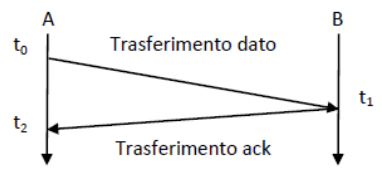
\includegraphics[scale=0.6]{ack}
\end{center}
Consideriamo i soggetti per il calcolo del tempo:\\
- Jitter: varianza sul delay, in particolare è la varianza sul ritardo \(Tx\). Cadenza di tempo di ricezione dei pacchetti; è particolarmente influente in connessioni real-time\\Per mitigare il jitter inseriamo un buffer in lato ricezione.\\
- \(t_{propagazione} \): tempo che il pacchetto impiega per arrivare a destinazione attraverso il mezzo\\
- \(t_{coda} \): è il tempo di permanenza in coda nel nodo (sia input che output), \emph{trascurabile}\\
- \(t_{elaborazione} \): è il tempo che serve al nodo per decidere su quale strada inoltrare il pkt \emph{trascurabile}\\
\begin{center}
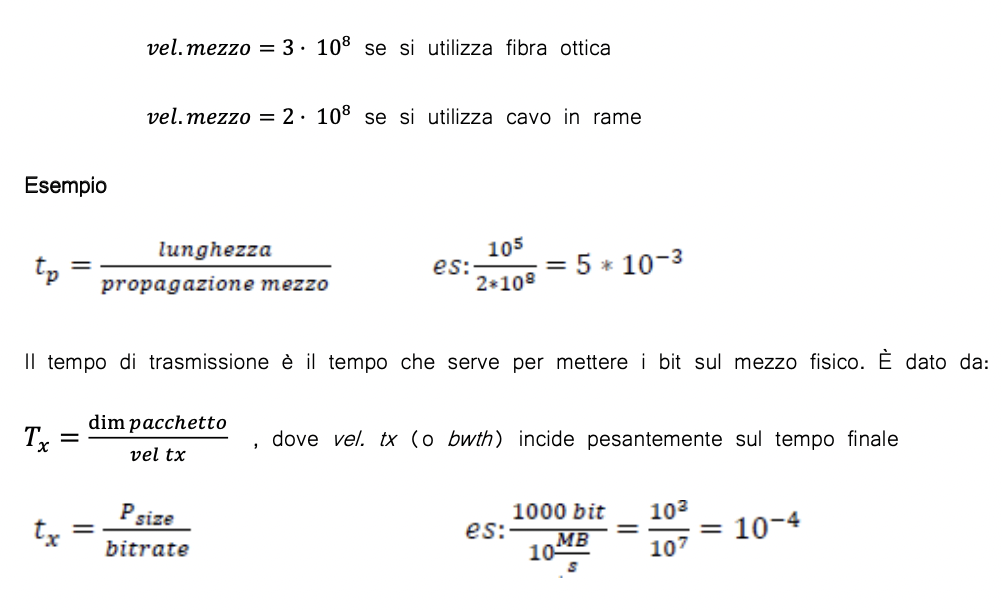
\includegraphics[scale=0.6]{3}
\end{center}

Consideriamo ora il singolo pacchetto:
Consideriamo un messaggio, esso può essere scomposto in dimensioni uguali, questi frammenti possono essere caricati su "pacchetti". Questo ci permette di gestire un \emph{n numero} di pacchetti di dimensione omogenea. 
I pacchetti hanno una propria autonomia, sono indipendenti l'un l'altro, sono tutti di dimensione uguali e sono formati da:
\begin{itemize}
\item Sorgente e destinatario
\item Sequence number o numero di pacchetto
\item Pacchetto
\end{itemize}
L'insieme sorgente, destinatario e sequence number va a formare l'header (intestazione), mentre il pacchetto va a formare il payload, ovvero il campo dati\\
\begin{center}
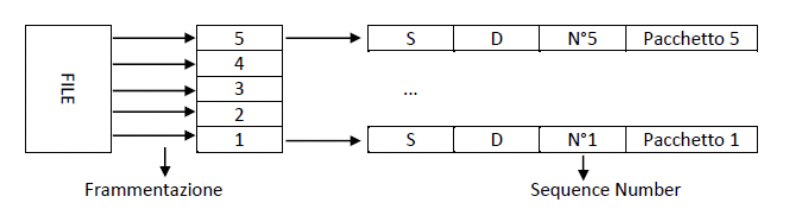
\includegraphics[scale=0.6]{package}
\end{center}
\section*{Comunicazione client-server, protocolli e HTTP}
Gli algoritmi di rete sono chiamati protocolli. I protocolli sono un insieme di regole condivise che vanno a regolare, in questo caso, le comunicazioni di rete.\\\\
Quando parliamo di funzione di rete facciamo riferimento alle funzionalità che ogni componente all'interno di un sistema di rete va a contribuire.\\
l'http è un protocollo di comunicazione, standardizzato, nato per far comunicare due componenti applicativi, che rappresentano lo user ed il server. (In essenza è un protocollo di trasferimento file -html-).\\
I client ed il server comunicano utilizzando funzioni di \emph{send<rq>}, spostandosi da stato di idle, e waiting for \emph{Rq}. E' fondamentale sincronizzare l'esecuzione delle macchine. I messaggi che si scambiano lo user ed il server sono standardizzati secondo il protocollo http.
\begin{figure}[H]
\begin{subfigure}[h]{0.5\linewidth}
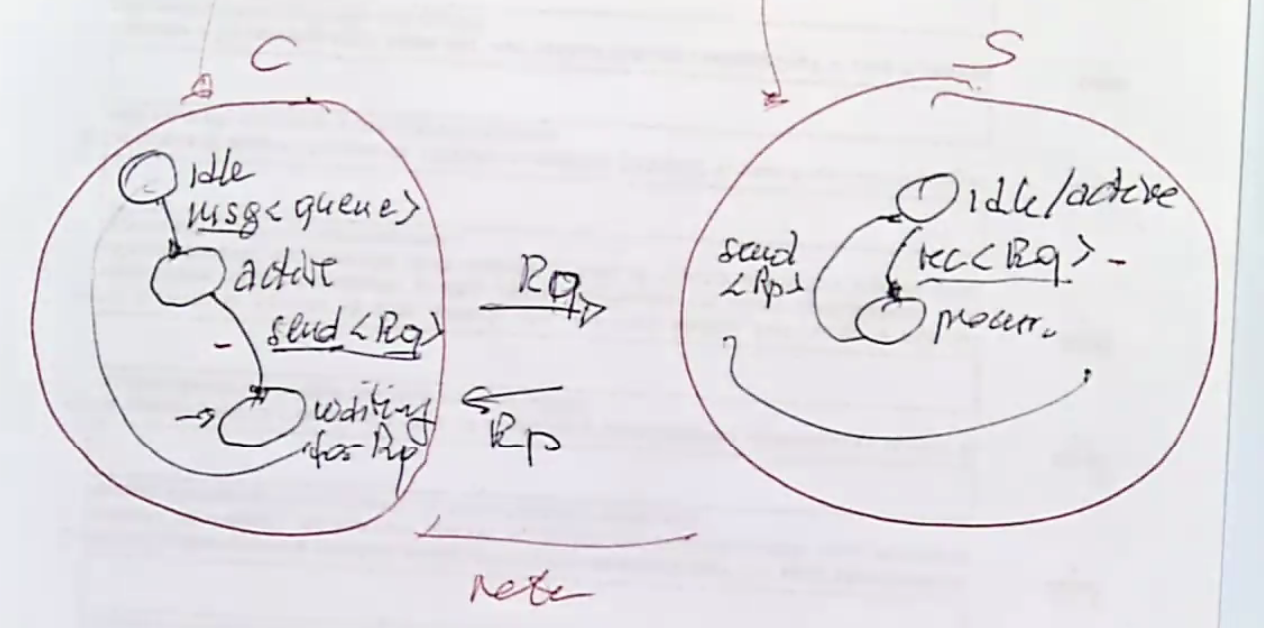
\includegraphics[width=\linewidth]{cs}
\end{subfigure}
\hfill
\begin{subfigure}[h]{0.4\linewidth}
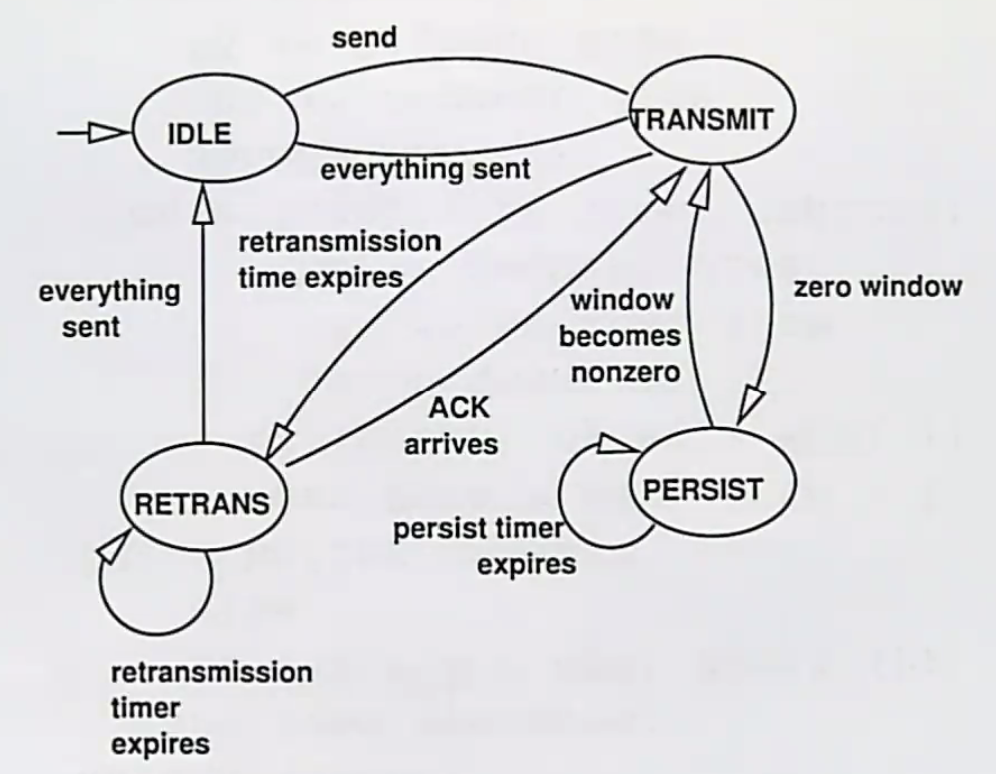
\includegraphics[width=\linewidth]{cs2}
\end{subfigure}%
\end{figure}

E' plausibile che sia il lato client che il lato server implementino buffer per gestire in maniera più efficiente le interfacce di rete.\\
Per ogni sessione di rete viene allocata un'interfaccia di comunicazione per funzioni di rete dedicate, caratterizzate da un protocollo. \\\\
Ogni comunicazione di rete è caratterizzato da:\\
- il protocollo legato alla funzione che permette la comunicazione\\
è una specifica di un sistema distribuito (almeno 2), comune, standardizzato\\
- l'interfaccia di servizio: è interna al terminale\\\\
L'organizzazione dei componenti di reti è basata su un'architettura gerarchica, con 7 livelli gerarchici definiti secondo una standard creato dalla OSI (Open System Interconnection). Per internet i livelli gerarchici che ci interessano sono 5.
\begin{center}
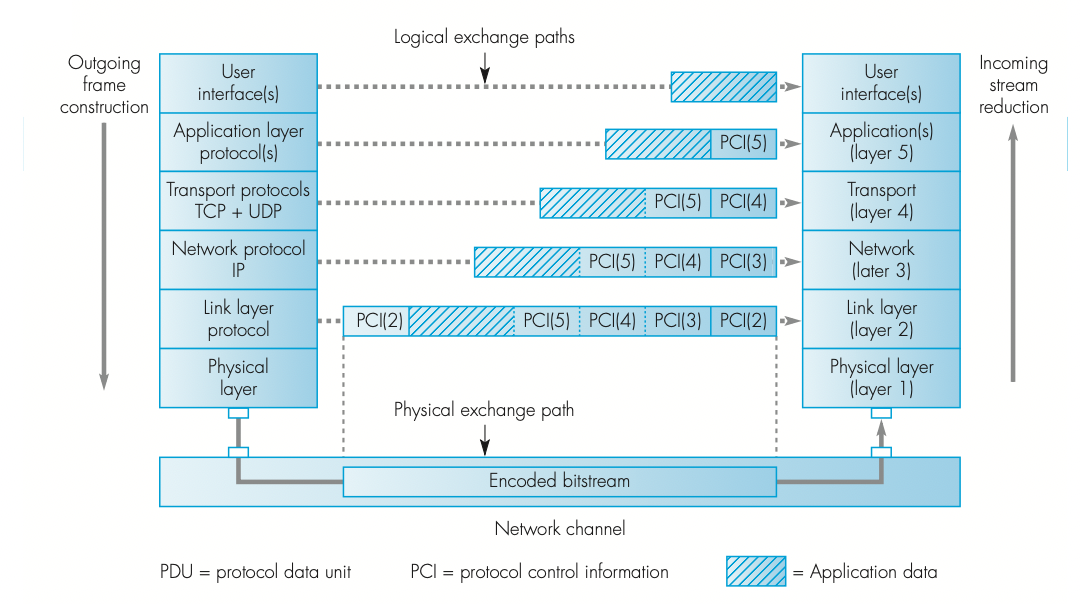
\includegraphics[scale=0.6]{osi}
\end{center}
La pila di protocolli è instaurata per ogni nodo connesso al sistema di reti, così come ad ogni terminale\\\\
Andiamo ad analizzarli secondo un bottom-up approach:\\
- Livello 1 | \textbf{Physical Layer}: si occupa di trasmettere bit lungo un canale di comunicazione (wired or wireless) secondo un dato clock sincronizzato alle due interfacce. Deve essere in grado di inviare e ricevere bit da un buffer (definito tra il livello 1 e 2).\\
- Livello 2 | \textbf{(Data) Link- Layer}: si occupa di definire i singoli pacchetti da trasmettere, fornisce un formato logico per organizzare la trasmissione da un nodo, ad uno adiacente ad esso. La quantità di data link è dato dal numero di archi uscenti da un dato nodo.\\
- Livello 3 | \textbf{Network (Protocol) Layer}: si occupa della funzione di instradamento (routing) e indirizzamento (addressing), non lavorano a livello link, ma sull'intera topologia di rete. Quando quindi si parla di IP o routing, si fa riferimento al livello 3.\\\\
Superiore a questi livelli abbiamo protocolli che permettono la comunicazione tra il router e l'applicativo utente\\\\
- Livello 4 | \textbf{Transport (protocols) Layer (TCP + UDP)}: si occupa di garantire l'affidabilità, è basata su una comunicazione end to end: in particolare i protocolli livello. L'UDP è un protocollo che non garantisce l'affidabilità, ma è più veloce. La scelta del protocollo da adottare è dato dal protocollo di livello 7. Si occupa anche di gestire l'ordinamento dei pacchetti\\
- Livello 4.5: Le socket sono delle primitive di comunicazione che si occupano di specificare sessioni tra processi applicativi utente.\\
- Livello 7 | \textbf{Application layer}: comprende per esempio l'http, file cluster, emails, è il livello più vicino all'utente\\\\
In Internet il livello 5 e 6 non sono stati implementati; questi 5 livelli gerarchici vanno ad implementare Internet.\\\\
Per completezza, il modello OSI descrivere anche i livelli 5 e 6:\\
- Livello 5 | \textbf{Session layer}: si occupa di gestire l'instaurazione, mantenimento, sincronizzazione delle sessioni applicative di un sistema.\\
All'interno di internet questo livello è affidato al livello 4.5, ovvero le socket.\\
- Livello 6 | \textbf{Presentation layer}: si occupa di organizzare i dati e di definire formati omogenei dati e gestire la crittografia \\\\
I router sono basati sui primi 3 livelli. Per comunicare, un user (dotato di livelli 1-4 + 7)  genera una request ad un server (1-4 + 7), che passa i vari router fino a raggiungere il destinatario, passando per le interfacce dei vari livelli, man man aggiungendo i vari header. Da notare che a livello 3 il modulo è singolo \\
\begin{center}
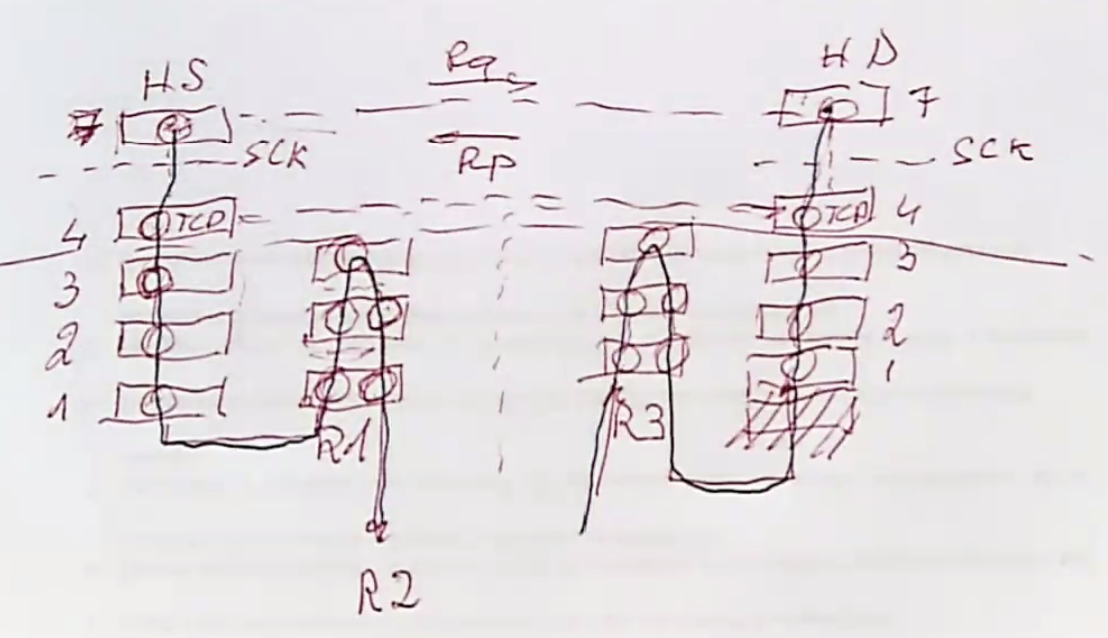
\includegraphics[scale=0.7]{req}
\end{center}
I livelli dal 4 compreso in sù sono chiamati end-to-end. La comunicazione tra livelli avviene solo \emph{peer-to-peer}, ogni livello conosce il funzionamento del livello \emph{n-1} in quanto si occuperà del trasferimento.\\
Il percorso a ritroso dei protocolli rimuove gli header di ogni livello precedentemente aggiunti, facendo arrivare il solo payload all'applicativo utente.\\\\

\section*{Data Link Layer}
All'interno di ogni nodo, ci sono \emph{n entità} per ogni arco uscente dal nodo. Il nodo A ha anche un link per la macchina host, ed il nodo E ha un link per l'host 2.
\begin{center}
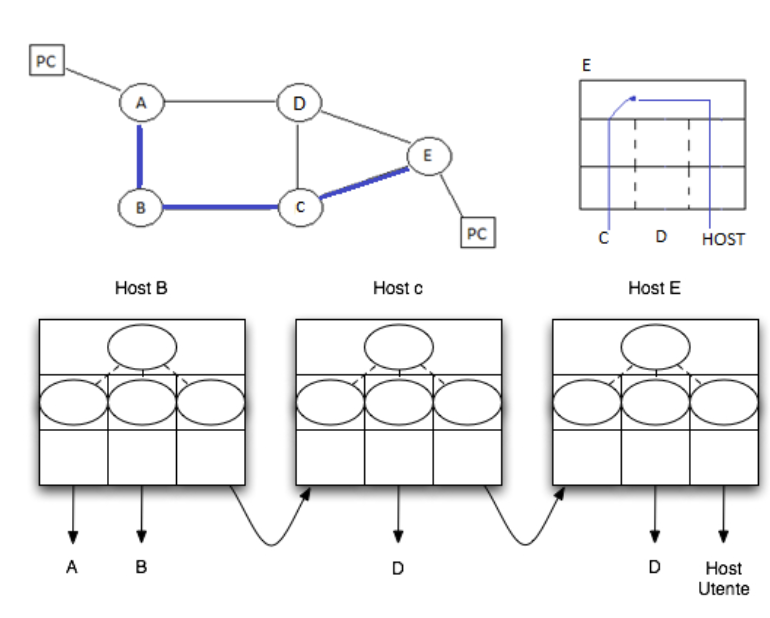
\includegraphics[scale=0.5]{dll}
\end{center}
All'interno del pacchetto è già salvato il percorso da prendere, mappato dal livello 3, che conosce tutta la rete.\\
I principi su cui si concentra il livello 2 sono il best-effort e l'affidabilità. \\\\
\emph{Come fa il canale a distinguere l'idle (continuo 5v o 0v) da una comunicazione effettiva?}\\
Viene introdotta una sequenza di bit che mi informa che l'inizio e la fine di una comunicazione. Queste sequenze sono chiamate \textbf{flags} di inizio e fine, e sono rappresentate dai bit 01111110, in particolare:\begin{center}
\{01111110 --- pacchetto dati --- 01111110\}\\
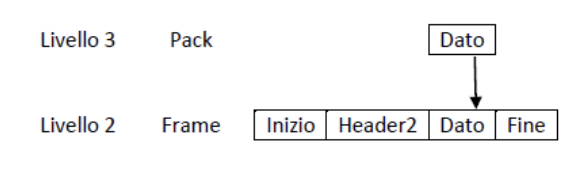
\includegraphics[scale=0.5]{dll2}
\end{center}
Per distinguere tra flags e sequenze bit è stato introdotto il bit stuffing.\\\\
\emph{Bit Stuffing}\\
Attraverso il bit stuffing, è introdotto un counter che, quando rileva 5 bit consecutivi con valore 1, viene introduce uno 0. Questa operazione è svolta dalla porta di I/O a livello firmware\\
Per esempio \emph{F--01111110--F diventa F--011111\textbf{0}10--F}.\\
Questo comporta che l'unico caso in cui il livello possa incontrare 5 bit di 1 consecutivi sia nel caso di flags. Quando le flags arrivano nell'altro capo del canale di comunicazione sono rimosse.\\\\
\emph{Come introduciamo l'affidabilità nel protocollo di livello 2?}\\
Dobbiamo assicurare la non duplicazione dei pacchetti, ordine nella ricostruzione e integrità. Per garantire ciò viene utilizzato un metodo chiamato \textbf{ARQ} ovvero lAutomatic Repeat Request, che permette la ritrasmissione del pacchetto fino alla conferma della ricezione.
Un esempio di esecuzione classico è il seguente:
\begin{center}
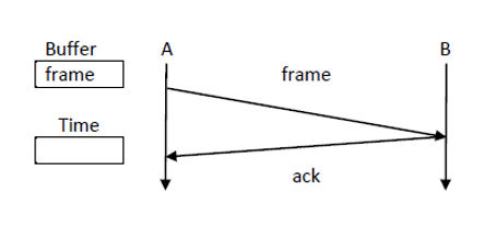
\includegraphics[scale=0.6]{l2}
\end{center}
Il sender A ha nel buffer il frame da inviare, che viene eliminato qualora riceve il messaggio di ack da parte del destinatario. Quando un messaggio di ack è ricevuto, il timer è riavviato. Se dopo un tempo \emph{t} il messaggio di ack non è ricevuto, il messaggio è ricopiato dal buffer e re-inviato.\\\\
Tuttavia è possibile che vi siano problemi in questo processo:\\
- Se per esempio il messaggio di ack è inviato troppo tardi ed il time-out avviene prima dell'arrivo è possibile che il messaggio di ack arrivi dopo la ritrasmissione.\\
E' quindi necessario implementare un numero progressivo rappresentato da una variabile \emph{V}, in particolare \emph{VS Variabile Sender}per identificare i frame. Se un frame è inviato più volte è compito del ricevente scartare il frame superfluo.
\begin{center}
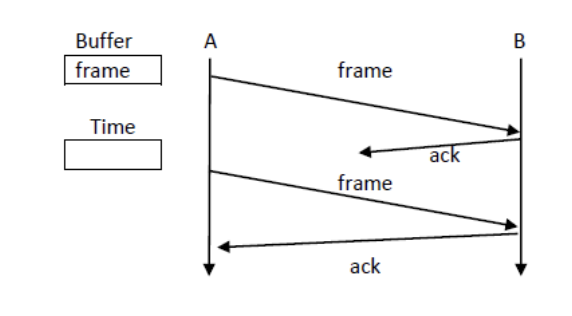
\includegraphics[scale=0.6]{ack1}
\end{center}
- Se invece il RTT (Round-trip-time) è desincronizzato?
\begin{center}
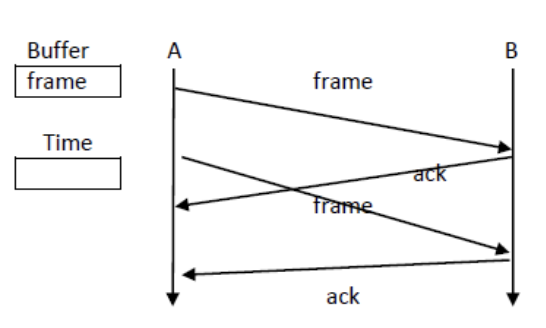
\includegraphics[scale=0.6]{ack2}
\end{center}
In questo esempio, ack arriva, ma il frame è già stato reinviato. Vengono quindi reinviati due frame uguali, e gli ACK riceventi fanno computare due volte il mittente. Il frame è scartato dal destinatario, ma la sincronizzazione è persa. \\
Allora per ogni ACK ricevuto, il mittente, controlla che sia l’ACK della stessa classe del pacchetto precedentemente mandato e se arrivano due ACK della stessa classe il mittente ignora il secondo (ridondanza). Conviene quindi implementare un variabile di sequenza anche per l'ACK \emph{VR Variabile Receiver}.\\\\

Una metrica per valutare l'efficienza è l'utilizzo del canale di connessione. U è l’utilizzo totale della rete: più il valore è alto, meglio viene usato il canale.\\
\emph{Come possiamo migliorare l'efficienza? }\\
Il nostro canale di comunicazione rimane fermo per molto tempo in attesa dell'ack. E se invece il protocollo non aspettasse l'arrivo dell'ack prima di inviarne un altro?\\
Potremmo migliorare di molto il tempo di trasferimento, ma complichiamo molto il protocollo.
\begin{figure}[H]
\begin{subfigure}[h]{0.5\linewidth}
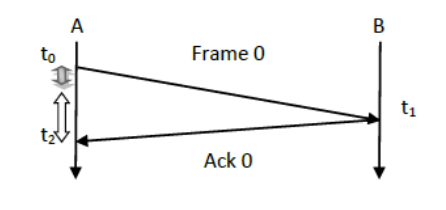
\includegraphics[width=\linewidth]{dll3}
\end{subfigure}
\hfill
\begin{subfigure}[h]{0.4\linewidth}
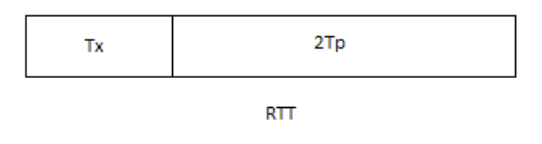
\includegraphics[width=\linewidth]{dll4}
\end{subfigure}%
\end{figure}
In questo esempio \(t_0\) rappresenta 1/3 del RTT, potenzialmente potrei inviarne altri 2.\\
Maggiore è il valore del tempo di propagazione, minore è la quantità di pacchetti inviabile in un singolo RTT, se tuttavia aumentiamo il più possibile il RTT, possiamo migliorare l'utilizzo.\\
Vediamo un esempio:
\begin{center}
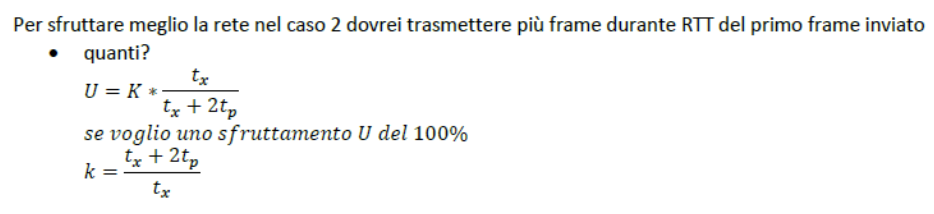
\includegraphics[scale=0.8]{ex3}\\
\emph{k rappresenta il numero di pacchetti che il trasmettitore è in grado di inviare senza aspetta l'ack. Più alto il rapporto, minore il k}
\end{center}
\begin{figure}[H]
\begin{subfigure}[h]{0.4\linewidth}
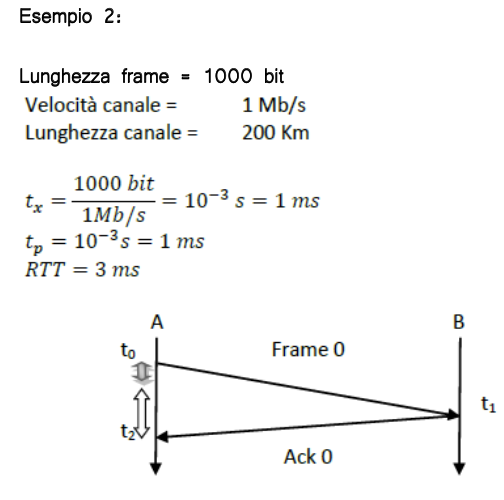
\includegraphics[width=\linewidth]{ex1}
\end{subfigure}
\hfill
\begin{subfigure}[h]{0.4\linewidth}
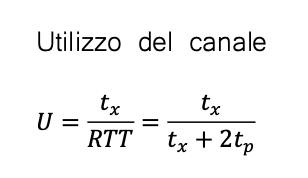
\includegraphics[width=\linewidth]{ex2}
\end{subfigure}%
\end{figure}
Questo modello è chiamato \emph{a finestra}, in cui nel tempo $T$ vengono inviati $n$ pacchetti senza attendere l'ack. Il prezzo da pagare è un buffer di trasmissione più grande.
\begin{center}
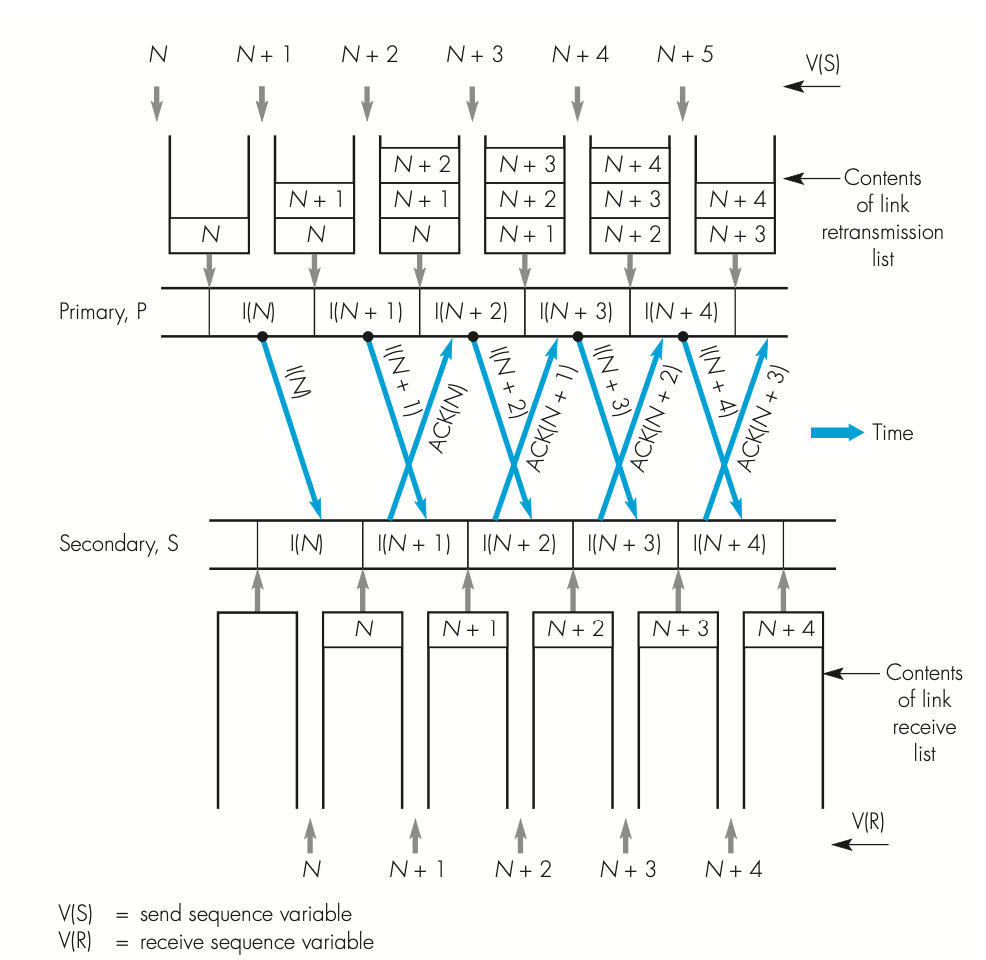
\includegraphics[scale=0.5]{m1}\\
\emph{Sender è sopra, receiver è sotto, il diagramma è ruotato di 90° a sinistra dal solito}
\end{center}
\long\def\comment#1{\emph{Cosa succede in caso di errore?} \\
}
Come andiamo a garantire l'affidabilità in questo protocollo?
\emph{Tecniche per l'affidabilità:}
Tecniche per l'affidabilità
Vi sono 3 protocolli che garantiscono l'affidabilità a livello 2, usano il metodo ARQ (Automatic Repeat Request), che prevede la ritrasmissione del pacchetto dopp un tempo di timeout fino a quando il destinatario non ne abbia confermato la ricezione (con un ACK):
\begin{itemize}
\item Idle RQ (stop-and-wait ARQ)
\item Continuous RQ (protocollo a finestra): \\
- go-back-N \\
- selective repeat\\
\end{itemize}
\emph{Idle RQ}:\\
Se dopo un tempo $t_x$ $>$ $RT$ T, l'ACK non è ancora arrivato, il mittente reinvia il frame. Ogni frame ha un numero progressivo (numero di sequenza) partendo da 0, così il ricevente può sapere se ha già ricevuto quel frame. Il ricevente in ogni caso risponde con l'ACK, anche se ha già il frame in arrivo.\\ Se il RTT è dominato dal tempo di trasmissione, il mittente non può migliorare di molto la velocità totale.
Se invece domina il tempo di propagazione, il mittente può inviare k frame e ascoltare poi per gli ACK senza aspettare il primo ACK del ricevente per inviare un secondo frame.\\\\

\emph{Andiamo a vedere i modelli a finestra più nel dettaglio, si suddividono principalmente in 2:}
\begin{itemize}\item Go-back-N: se il ricevitore riceve un frame fuori posizione, scarta tutti i frame successivi indipendentemente dalla correttezza, richiedendo la ritrasmissione da parte del trasmettitore a partire dell'ultimo frame corretta.
\begin{center}
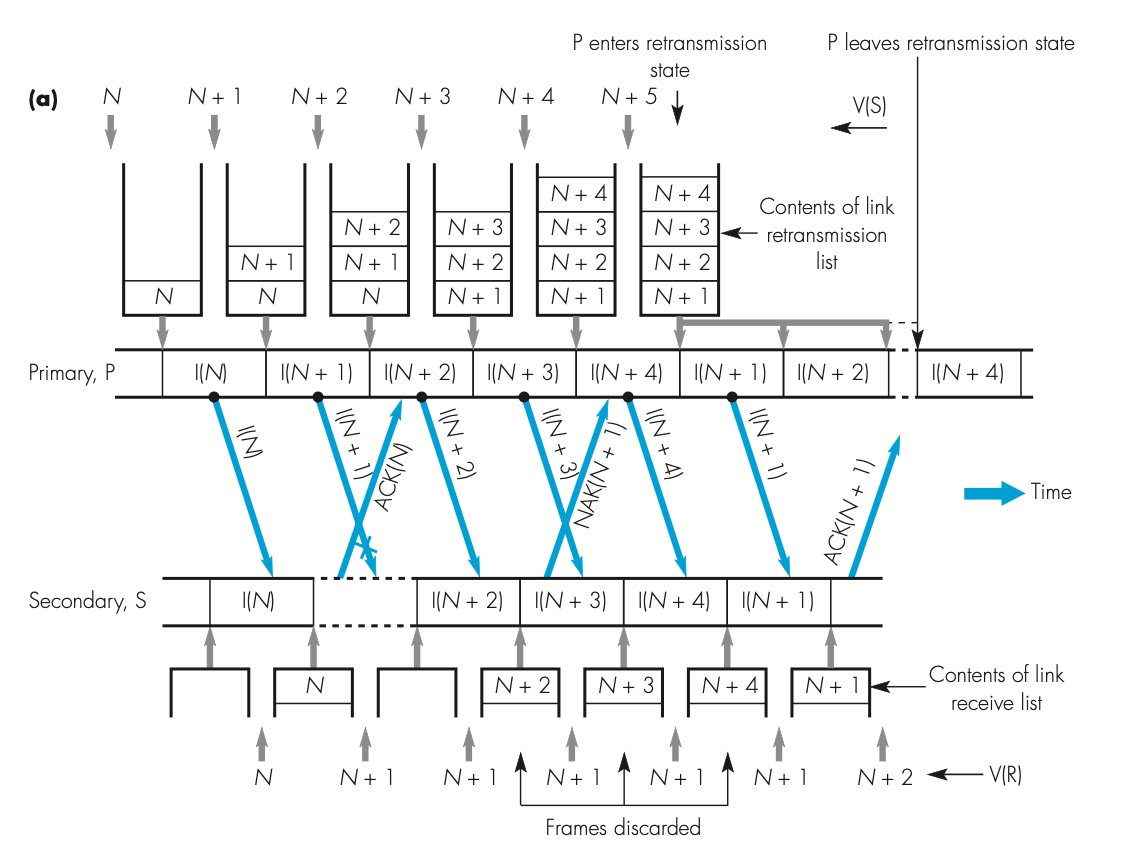
\includegraphics[scale=0.5]{nak}
\end{center}
In questo esempio il frame $n + 1$ non arriva correttamente a destinazione, vengono quindi scartati i frame $n +2, n + 3, n + 4$ in quanto il sender non ha modo di sapere che $n + 1$ non è arrivato.\\
Il receiver quindi manda il $NAK(n + 1)$, per richiedere la ritrasmissione a partire da $n+1$.
Al posto di implementare un $NAK$, riutilizziamo l'ACK, con indice l'ultimo frame corretto.\\
Il $NAK(n+1)$ è sostituito con $AK(1)$. Il buffer di ricezione è grande 1, o n.
\begin{center}
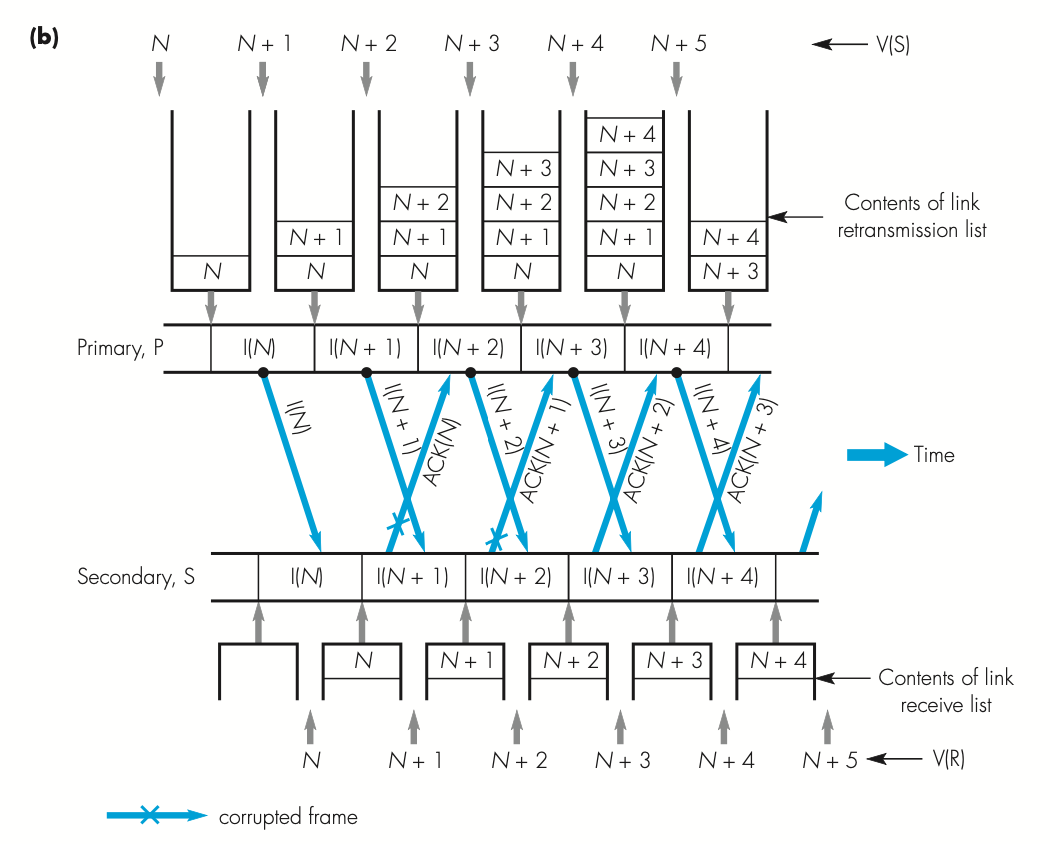
\includegraphics[scale=0.5]{nak2}
\end{center}
In questo esempio i problemi sorgono quando vengono inviati gli ACK. \\Gli $ACK(n)$ e $ACK(n+1)$ non arrivano, tuttavia arriva $ACK(n+2)$. 
\end{itemize}
Se ragioniamo con una logica selettiva, il sender dovrebbe reinviare i frame $n$ e $n+1$; se ragioniamo con una logica cumulativa il sender non reinvia niente in quanto comprende che fino a n+2 sono arrivate.
\begin{itemize}
\item Selected Repeat (ack cumulativo) (l'esempio sul libro ragiona con un ack selettivo):\\
È come go-back-N, ma non si reinviano tutti i frame ma solo quello errato. Serve quindi che il ricevitore abbia un buffer almeno di k elementi così da gestire gli altri frame in attesa del reinvio di quello errato.\\\\
Quando un frame $(n)$ non arriva, il receiver inoltra un $AK(n)$ per segnalare che ha bisogno dei frame a partire del pacchetto $(n + 1)$ (logica cumulativa) Il buffer di ricezione è grande quanto il buffer di trasmissione, ed è tenuta una copia di tutto ciò che è ricevuto correttamente.\\

\end{itemize}
In riepilogo:\\
- Go-Back-N \hfill windowSender: k \hfill windowReceiver: 1 \hfill nsequenzaMax: k+1\\
- Selected Repeat \hfill windowSender:k \hfill windowReceiver: k \hfill nSequenzaMax: 2k\\
- IdleRQ: \hfill windowSender: 1 \hfill windowReceiver: 1 \hfill nSequenzaMax: 2\\

\section*{Specifiche per protocolli basati su reti broadcast}
Nelle reti broadcast, a differenza delle reti LAN, i frame sono inviati a tutte le stazioni. E' compito dunque delle singole stazioni droppare il frame non necessarii. Questo approccio garantisce il \emph{fairness}, ma necessita di un alcuni meccanismi per garantire la sincronizzazione, e la gestione di un'eventuale perdita di token. La stazione delegata è chiamata stazione controllore.\\\\
I protocolli di accesso a canale condiviso sono suddivisi in base al tipo di accesso al canale condiviso, che può essere \textbf{deterministico} o  \textbf{casuale}\\
 Tuttavia da sistemi operativi sappiamo che un solo soggetto può entrare in sezione critica alla volta. \\
Dobbiamo andare ad implementare algoritmi di gestione per l'accesso condiviso:
\begin{itemize}
\item Token ring: un token è assegnato al soggetto che in quel momento è ha diritto di broadcast, quando il token è tornato al soggetto iniziale, sappiamo che il messaggio è stato inviato a tutti i soggetti. Il token è quindi rilasciato e dato alla prossima stazione. \\
Questo approccio garantisce il \emph{fairness}, ma necessita di un alcuni meccanismi per garantire la sincronizzazione, e la gestione di un'eventuale perdita di token. La stazione delegata è chiamata stazione controllore.
\item Aloha: è il primo protocollo probabilistico per l'accesso ad un canale probabilistico, basato su un modello broadcast (un satellite) (che ha un ping di 250ms). Tuttavia questo modello risulta particolarmente inefficiente, raggiungendo un picco del 18\%. Gli errori/corruzioni sono risolti ritentando il trasferimento. 
\item CSMA-CD (Carrier Sense Multiple Access/Collision Detection): è un modello basato su cavi (il ping è quindi basso, così come il tempo di propagazione)(efficienza tra il 90 e il 95\%). Il carrier verifica a priori che il canale sia vuoto, prima di inviare il frame. Più stazioni competono per l'accesso al canale; qualora il canale sia attualmente occupato, il nodo si mette in attesa prima di iniziare la trasmissione. Qualora la collisione sia rilevata, essa è gestita con l'algoritmo Binary Exponential Backoff, e la trasmissione è immediatamente fermata, diminuendo il tempo prima di un'eventuale ritrasmissione.\\\\
Il CSMA può avere più configurazioni, in particolare può essere 1-persistente (l'ascolto ed il tentativo di trasmissione è continuo) o non-persistente (i tentativi di ri-tramissione avvengono dopo un tempo casuale).\\
Il tempo casuale è in un range BEB (Binary Exponential Backoff): viene scelto un numero casuale tra $2^i-1$ (ove $i$ è il numero di collisioni avvenute )e lo si moltiplica per $51.2\mu s$, ovvero lo slot di tempo minimo.\\
Il protocollo LAN è definito all'interno del documento \emph{IEEE 802.3}, mentre il rpotocollo WIFI è definito nel \emph{IEEE 802.11}.
\end{itemize}
\emph{Codifica di Manchester}\\
In questa codifica imponiamo un cambiamento di stato per la codifica di 1 o 0:
\begin{itemize}
\item ogni bit valore 1 comporta una trasmissione in salita (da 0 a 1)
\item ogni bit di valore 0 comporta una trasmissione in discesa (da 1 a 0)
\item l'assenza di transizione è rappresentata dall'assenza di segnale
\end{itemize}
Siccome è possibile che due bit consecutivi siano di valore uguale, è necessario rendere possibile lo spostamento del valore all'alto o al basso senza emettere un output. Questa operazione di riposizionamento è chiamato \emph{logical zero (spostamento verso il basso) o logical one (spostamento verso l'alto)} e dura mezzo periodo del clock.
\begin{center}
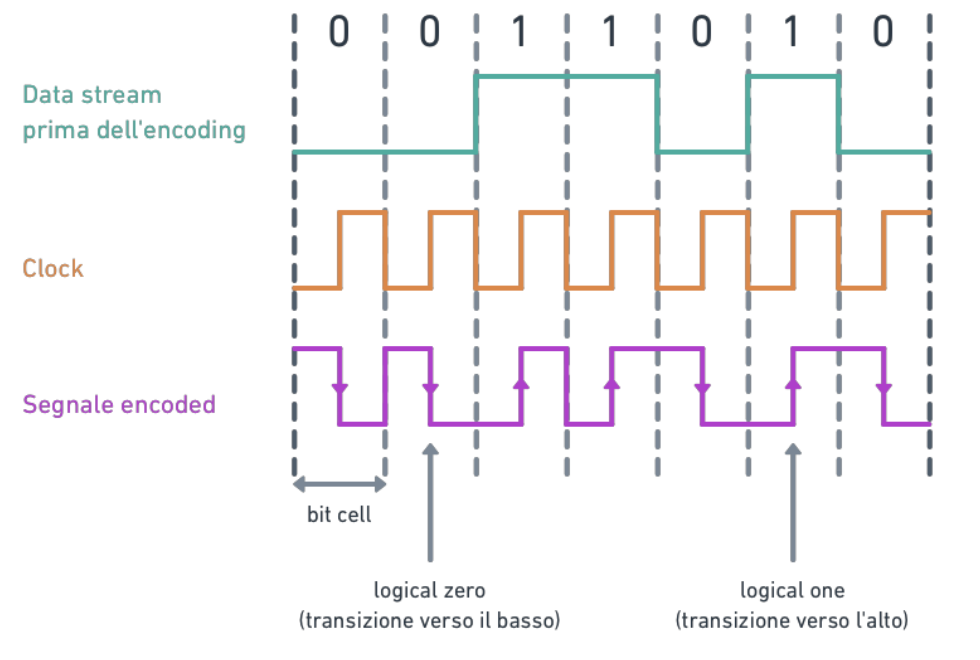
\includegraphics[scale=0.5]{manch}
\end{center}
L'obbiettivo della codifica è quello di permettere sia il trasferimento di dati, ma anche del periodo del clock. \\\emph{Ma come fa il ricevitore a distinguere effettivamente la durata del clock dalle transizioni di riposizionamento?}\\
Introduciamo il formato frame delle trasmissioni LAN.
\begin{center}
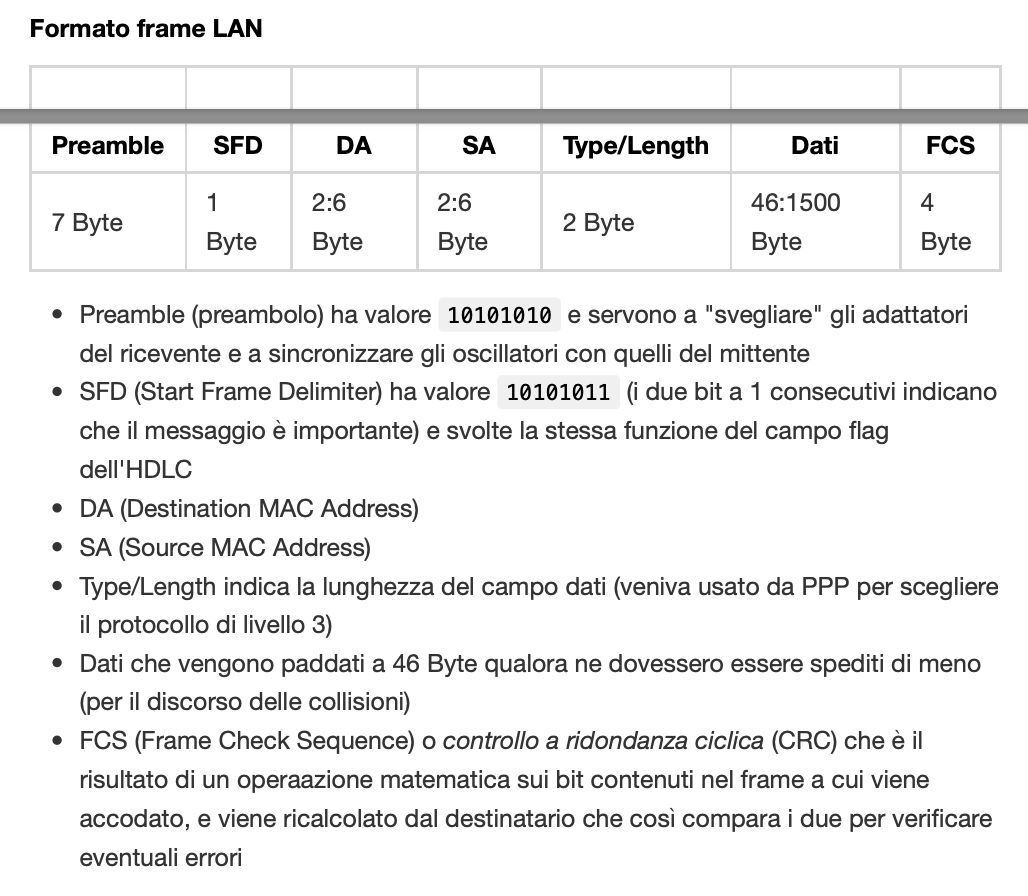
\includegraphics[scale=0.5]{format}
\end{center}
Il preambolo, in particolare, viene utilizzato per sincronizzare il gli orologi del mittente e del destinatario.\\\\
\emph{Sottolivelli del livello 2:}
Il livello 2 è suddivisibile in 2 porzioni:
\begin{itemize}
\item LLC: Logical Link Control, ovvero la parte superiore\\
Comune a tutti gli standard della famiglia IEEE 802
\item MAC: Media Access Control, ovvero la parte inferiore
\end{itemize}
\emph{Domini di collisione}\\
All'interno di una rete connessa con cavi, abbiamo una serie di componenti che insieme vanno a formare il dominio di collisione: ovvero il dominio di rete in cui i componenti competono per l'accesso alle canale.
\begin{itemize}
\item Hub: è un apparato passivo centro stella che riceve e ritrasmette i segnali (esegue una funzione di ripetitore), non interviene a livello due e non separata/crea domini di collisioni.
\item Bridge: è un operatore attivo, esegue il compito di suddividere domini di collisione, dividendoli in due sottodomini. Esso è dotato di una schede di rete con relativo indirizzo MAC, indirizza i pacchetti in entrata verso gli hub corretti, controllando che non siano corrotti.\\
Consideriamo la seguente immagine:
\begin{center}
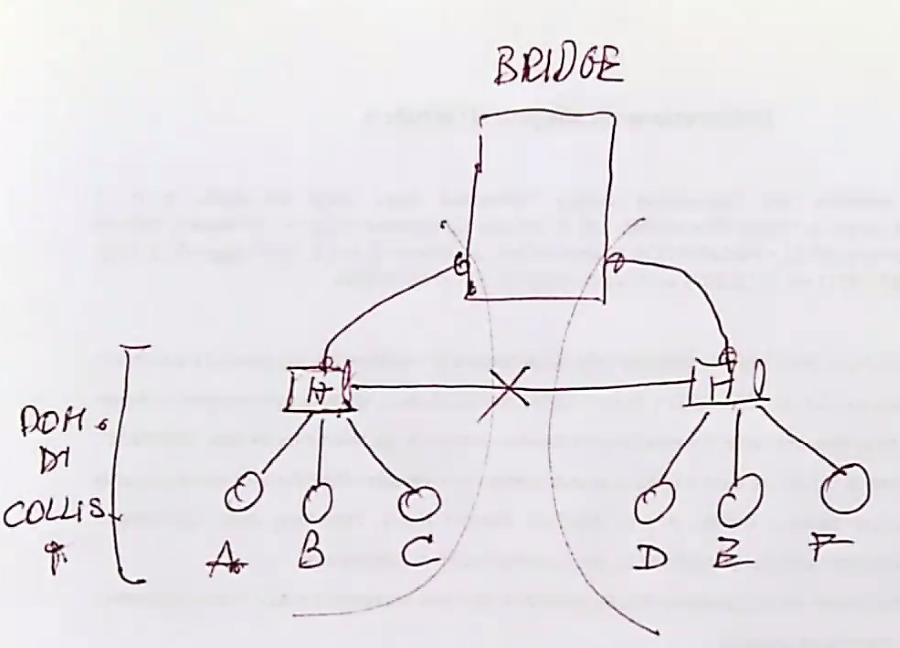
\includegraphics[scale=0.5]{bridge}\\
\emph{Il dominio di collisione è separato dal bridge, le collisioni all'interno delle singole porzioni possono comunque avvenire}
\end{center}
Quando un bridge riceve un pacchetto in entrata effettua un'operazione di "store and forward". 
Per instradare i pacchetti da un dominio ad un altro, il bridge utiliza una tabella di forwarding, se il pacchetto in entrata è indirizzato ad un nodo di un hub differente esso effettua un'operazione di forwarding.
\item Bridging hub: ha una funzione simile al repeater, ovvero quello di fornire l'interconnessione tra più repeater hubs. La differenza fondamentale è che il bridging hub ha svolge anche una funzione di store, e controllo di errori prima dell'inoltro. La presenza di un bridging hub è ininfluente a due stazioni comunicanti, per questo vengono anche chiamati "transparent bridges". \\
\begin{center}
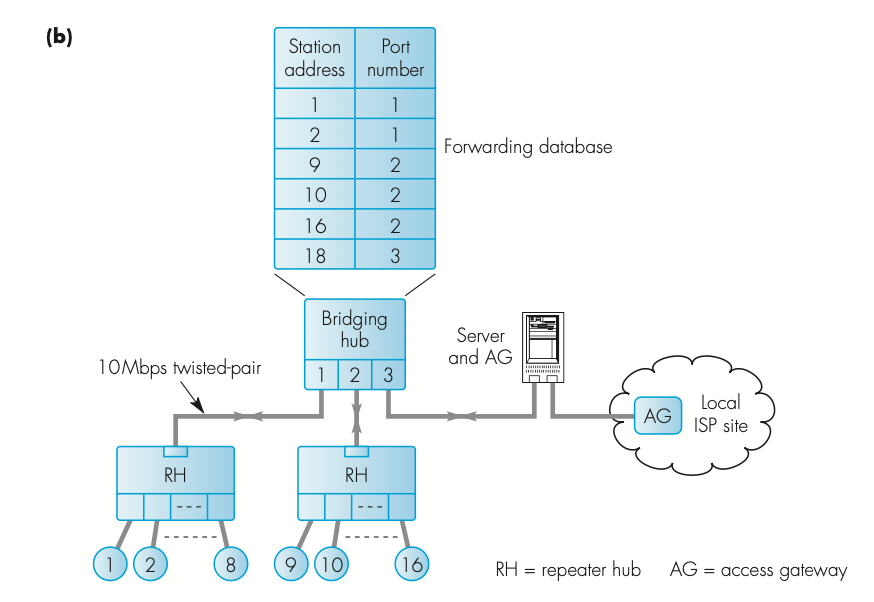
\includegraphics[scale = 0.6]{flooding}
\end{center}
Il bridge mantiene anche un forwarding database o routing directory, che registra, per ogni porta, la porta di uscita (se presente). Se un frame ricevuto indirizza all'hub di ricezione, esso viene scartato, altrimenti viene forwardato secondo ciò che è presente all'interno della table. Se nella table non è mai stata caricata una entry, il pacchetto viene forwardato su tutti i canali presenti (operazione di flooding).
La tabella è aggiornata dinamicamente, ma periodicamente deve essere anche flushata.
\item Switch: è come un bridge, ma non utilizza CSMA/CD ma le porte di input/output sono punto a punto (non più broadcast). Lo switch gestisce frame che arrivano contemporaneamente su porte di input diverse. Ho solo bisogno di garantire che le frame siano del tipo di CSMA/CD per quando verranno inoltrate nei vari domini.
\begin{center}
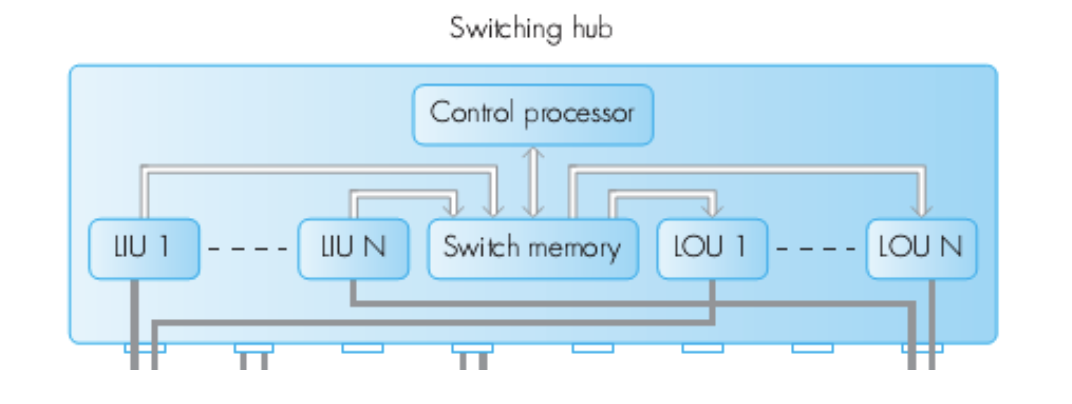
\includegraphics[scale=0.5]{switch}
\end{center}
\end{itemize}

\emph{Ethernet a 100 Mbps o 100Base4T}\\
100B4T è nato per incrementare la velocità di Ethernet portandola a 100Mbit/s utilizzando 4 cavi. Per fare ciò vengono utilizzate 4 coppie di cavi che consentono una trasmissione CSMA/CD bidirezionali.
\begin{center}
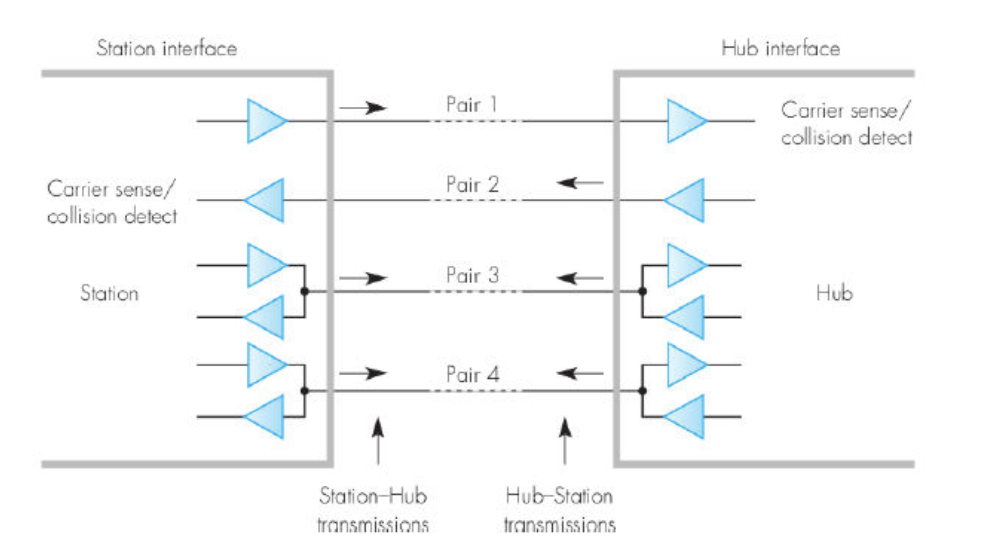
\includegraphics[scale=0.5]{eth}
\end{center}
\begin{itemize}
\item I cavi 1, 3, 4 si occupano della trasmissione.
\end{itemize}
Il rimanente cavo è utilizzato per rilevare le collisioni. Ognuno dei 3 cavi ha una velocità di 25 Mbps.\\
A questa velocità tuttavia non è applicabile la codifica Manchester, si utilizza una codifica chiamata \emph{8B6T} che converte 8 bit in simboli in base 3 applicando un cambiamento della fase del segnale che permette di trasferire dati a 100 Mbs
\begin{center}
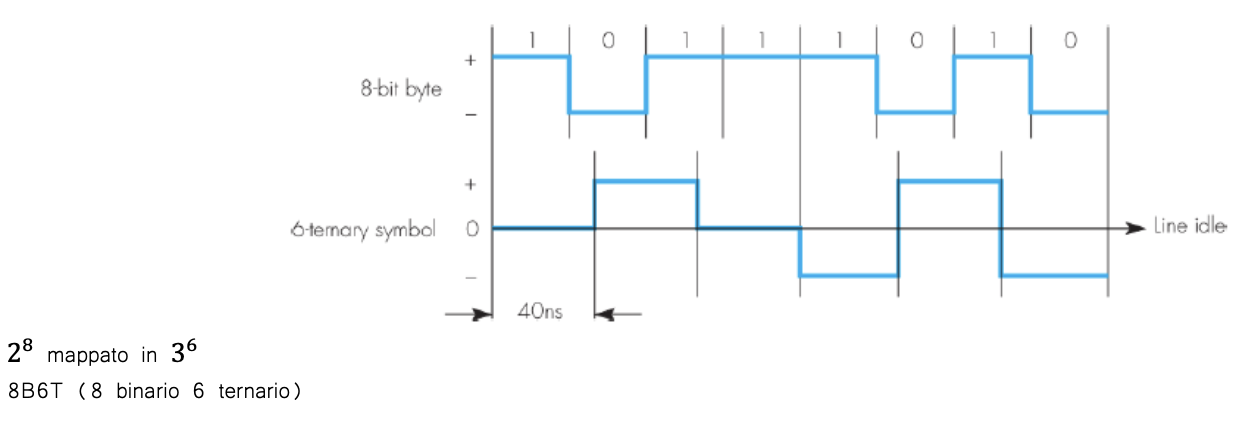
\includegraphics[scale=0.5]{eth2}
\end{center}

\textbf{Logical Link Control}\\
Come abbiamo specificato in precedenza, il livello 2, o mac layer, comunica con il physical layer attraverso l'interfaccia di scheda di rete. \\Dobbiamo tuttavia sottolineare che il livello 2 ha un ulteriore sottolivello, ovvero il \textbf{logical link control}. 
Il logical link control è costituito da connessioni logiche punto a punto indipendenti dai servizi sottostanti, dotati di servizi di trasmissione best effort e servizi affidabili. 
\begin{center}
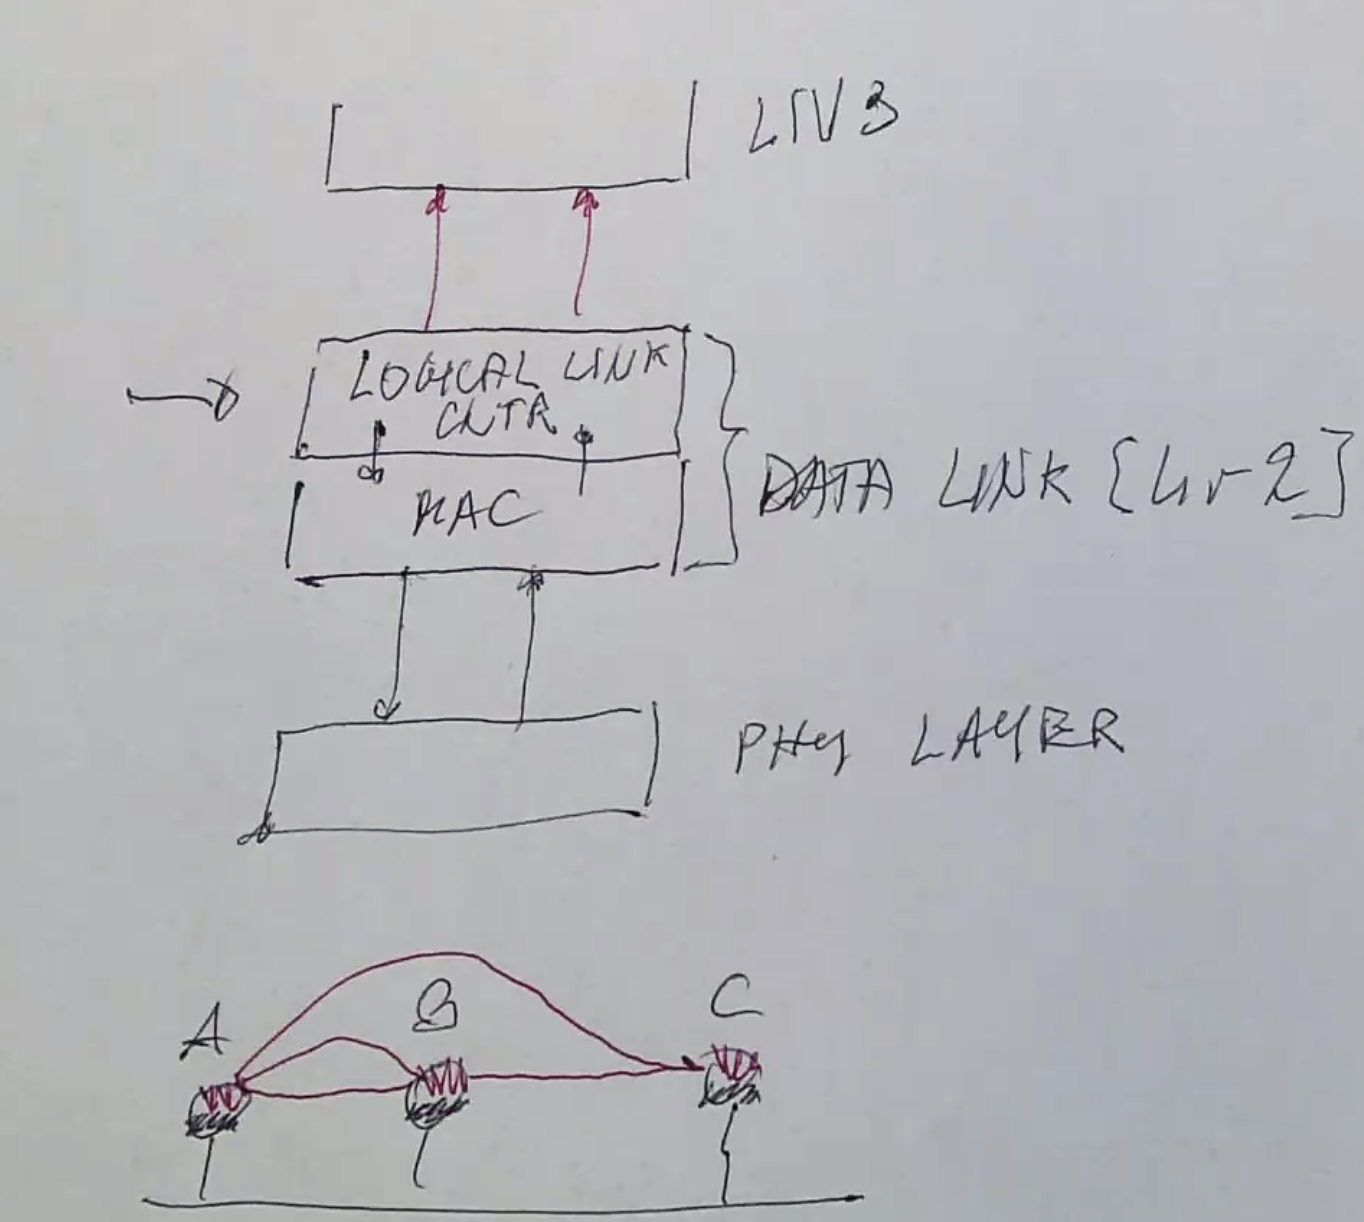
\includegraphics[scale=0.4]{llc}
\end{center}

\textbf{IP: protocollo a livello 3}\\
I frame diventano pacchetti, e fornisce un servizio non affidabile. L'intstazione del pacchetto è organizzata in 5 parole da 32 bit, con un campo opzionale.
\begin{center}
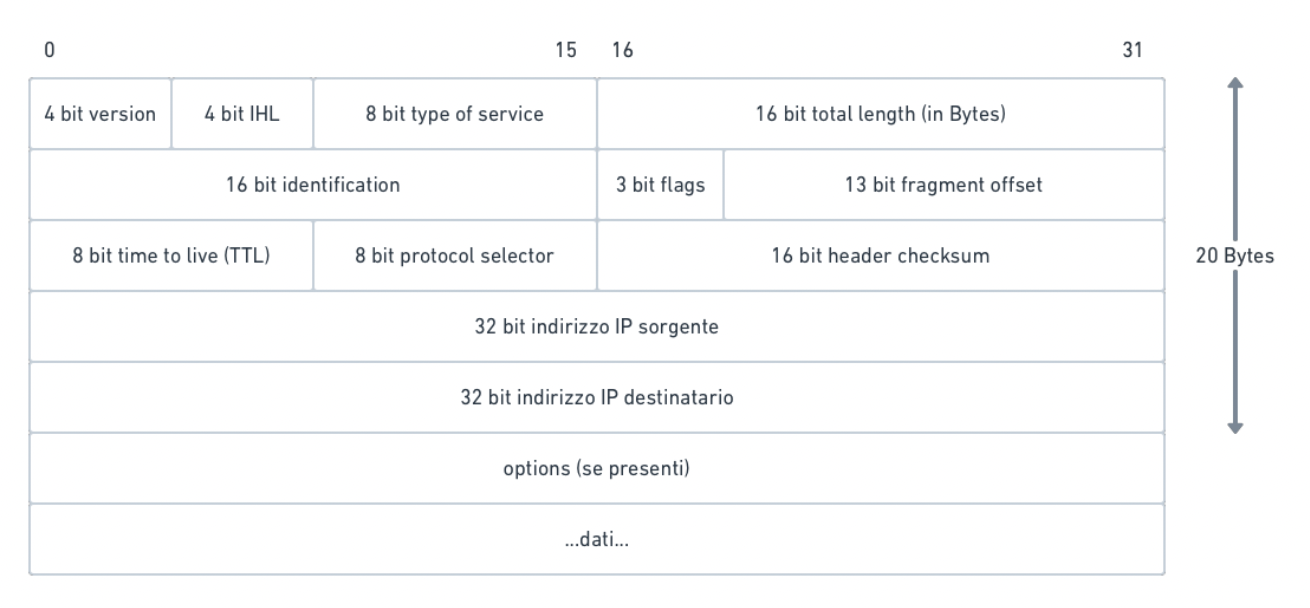
\includegraphics[scale=0.5]{ip}
\end{center}
\begin{itemize}
\item Version, specifica la versione di IP (in questo caso 4) e istruisce quindi gateway,
router e host su come interpretare il pacchetto
\item IHL (Internet Header Length), la lunghezza dell'header può essere variabile (campo opzionale), in multipli di 32 bit. Il minimo è 5, il massimo è 15
\item ToS (Type of Service), fornisce una priorità al pacchetto IP, cosicchè i router possano instradarlo nel modo migliore
\item Total Length, indica la lunghezza totale del pacchetto, compresa intestazione e dati. La dimensione massima è $2^{16}$ - 1 = 65535
\item Parola di 32 bit per la frammentazione dei pacchetti\\
- Identification, identificatore del pacchetto originale, uguale per ogni pacchetto di un singolo messaggio\\
- 3 bit Flags, composti da un bit riservato, uno DF (Don't Fragment) per indicare di farlo passare in una rete che lo può spostare intero e uno MF (More Fragment) a 1 quando devono essere inviati ancora dei pacchetti, a 0 quando è l'ultimo\\
- Fragment offset, indica quanti bit sono già stati inviati dai frammenti precedenti; non vengono contati i bit ma gruppi di 8 Byte, massimizzando così l'uso di questi 13 bit (non esiste quindi un frammento più piccolo di 8 Byte). Indicizza 213 = 8192 gruppi di 8 Byte, quindi 65536 Byte (che è la maximum segment size di un segmento di livello 4)\\
\item Parola di 32 bit per controllo\\
- Time To Live (TTL), tempo massimo di vita di un pacchetto nella rete; se, scaduto questo tempo, il pacchetto non è stato consegnato, e va eliminato. Di solito indicato come numero di hop (Hop To Live)\\
- Protocol Selector, indica il protocollo di livello 4 usato dal mittente, cosicchè il destinatario possa passarlo allo stesso protocollo\\
- Header Checksum, usato per efficienza operativa, poichè se la checksum è sbagliata evito subito di instradare il pacchetto (verifica integrità solo per la parte dell'intestazione, per questo il livello 4 ricalcolerà la CRC anche per il contenuto IP)
\item Options, campo opzioni variabile, nel quale vengono specificate opzioni su: sicurezza, source routing, ...
\end{itemize}
L'IPv4 ha un'indirizzamento a 32 bit, quindi gli indirizzi sono $2^{32}$, ogni macchina connessa ad internet internet è indirizzabile ad un indirizzo IP univoco.\\\\
\textbf{Frammentazione e ricostruzione pacchetto IP}\\
Supponiamo di dover trasferire un pacchetto di 7000 Byte da una LAN token ring attraverso internet fino ad un host di una LAN ethernet. Assumiamo che la quantità massima di trasmissione (MTU) sulla rete token ring sia di 4000 Byte, mentre quella ethernet di 1500 Byte. IP aggiunge altri 20 Byte di intestazione quindi:
\begin{itemize}
\item abbiamo a disposizione 4000 - 20 = 3980 Byte per l'invio
\item dobbiamo creare frammenti con payload multipli di 8 Byte per l'invio (attraverso un indice tengo conto di quanto ho inviato)
\item vengono inviati due frammenti (3976 e 3024 Byte), che passano attraverso internet
\item arrivano alla rete ethernet dove devono essere frammentati di più perché la quantità massima di trasmissione qui è di 1500 Byte (1500 - 20 = 1480 Byte) \item ogni pacchetto che arriva viene frammentato in altri 3 pacchetti (1480 - 1480 - 1016 Byte il primo, 1480 - 1480 - 64 Byte il secondo)
\end{itemize}
I pacchetti non sono riframmentati da IP, ma la ricostruzione avviene a livello end-user.

\section*{Subnetting} 
I router non possono avere una tabella di routing contenente tutti gli host, dato che le classi di indirizzamento (sono troppi). Per mitigare questo problema ogni router di una sottorete conosce gli indirizzi degli host a lui collegati e quelli dei router a livello superiore.\\
I router dei livelli superiori non tengono traccia di tutti gli indirizzi degli host delle sottoreti collegate, bensì si suddivide il net id, creando un subnet id (oltre il net id) che permette di verificare se un indirizzo fa parte di una delle sottoreti senza conoscerne gli host. \\In pratica:
\begin{itemize}
\item il router controlla che il net id del destinatario sia uguale a quello delle sue sottoreti \\
- se si, si controlla a quale sottorete inoltrare il pacchetto in base al subnet id \\
- se no, il pacchetto non viene inoltrato nelle sottoreti collegate al router\\
\item il router della subnet a cui arriva il pacchetto inoltrerà il pacchetto all'host corretto
\end{itemize}
Il subnet id è sempre ricavato da una parte della parte host dell'indirizzo. \emph{Come facciamo a capire quanti bit sono stati assegnati al subnet id?} Viene utilizzata una \emph{subnet mask}.
Per capire a quale sottorete deve essere indirizzato il pacchetto, viene fatto un AND logico con la subnet mask, formata da tutti 1 nella porzione net id e subnet id e 0 altrove. Il subnet mask ci permette di aumentare la vita del protocollo iPv4, permettendo l'utilizzo di più indirizzi.
\section*{CIDR | classless inter domain routing}
E' il contrario dell'indirizzamento a classe, gli spazi di indirizzamento sono organizzati in classi di indirizzamento per regione (Asia, Europa, America etc.)
Per esempio la classe di indirizzamento per l'europa è
\begin{center}
194.0.0.0 - 192.255.255.255\\
195.0.0.0 -  195.255.255.255\\
\emph{256 (primi 3) * 256 = 65536 + 65536 = 131.072 possibili combinazioni}\\
\emph{131.072 * 256 = 33.554.432 hosts, possibili indirizzi}
\end{center}
Una qualsiasi organizzazione può fare richiesta per l'assegnamento di un indirizzo base, con un  range di indirizzi utilizzabili. Questo meccanismo è complementato dall'utilizzo del subnetting con le masks.
\section*{NAT | Network Address Translation}
Ad ogni dispositivo collegato all'interno di una rete viene assegnato un indirizzo privato, che permette l'identificazione all'interno della rete. L'indirizzo NAT è pubblico, univoco in tutto il pianeta. Quando un host vuole comunicare con l'esterno, il servizio NAT rimpiazza l'indirizzo privato con un indirizzo pubblico all'interno della sottorete, e l'associazione è salvata all'interno di una tabella. All'interno della tabella sono salvate:
\begin{center}
$<ip$ $interno, porta$ $interna, ip$ $esterno, porta$ $esterna, ip$ $destinazione, porta$ $nat>$
\end{center}
Questo meccanismo serve anche a proteggere le macchine interne dall'esterno, fungendo anche un compito di firewall.
\begin{center}
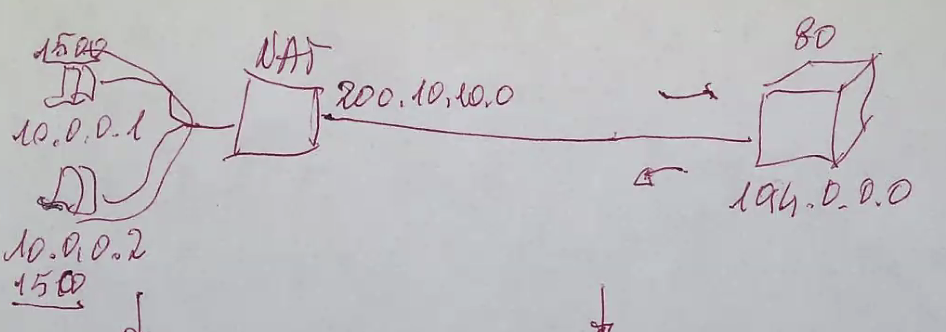
\includegraphics[scale=0.5]{nat}
\end{center}
Quando un server restituisce una reply, il pacchetto è complementato con la porta NAT associata al terminale che ha fatto la richiesta, il NAT svolge poi il matching per ricavare l'indirizzo privato.\\
Se un dispositivo interno (per esempio un sito web) volesse esporsi al pubblico, potremmo assegnargli un ip pubblico accessibile dall'esterno, o configurando una porta aperta (se per esempio è 80, sappiamo che è un sito web).
\section*{ARP | Address Resolution Protocol}
Questo meccanismo a livello 2 si occupa di mappare un indirizzo IP ad un corrispondente indirizzo MAC Utilizzando un $IP_b$ il protocollo ARP un host può comunicare con un altro host all'interno della rete un ARP request inviandolo a tutti in un broadcast request.\\
Quando un host con $IP_a$ deve effettuare una comunicazione ad un host con $IP_b$, viene effettuata una \emph{ARP Request}. \\L'ARP Request è effettuata a tutti gli host all'interno della rete, e contiene \begin{center}
MAC sorgente, $l'IP_a$, l'indirizzo IP del destinatario
\end{center} Attraverso questa trasmissione broadcast, se l'host è all'interno della rete viene effettuata una \emph{ARP Reply}, destinato al MAC dell'host sorgente, contente il proprio MAC.\\
Ogni volta che la richiesta MAC termina con successo, l'indirizzo MAC richiesto/inviato viene salvato all'interno di una ARP Cache, che mappa gli indirizzo $IP_i$ con gli indirizzi $Mac_i$.\\
\emph{RARP | Reverse ARP}\\
E' una variante di ARP, utilizzato quando un host conosce il proprio MAC ma non conosce il proprio IP. Viene creata una tabella che contiene tutte le coppie MAC-IP degli host.



\section*{DHCP | Dynamic Host Configuration Protocol}
E' un meccanismo utilizzato per richiedere ad un server DHCP un IP dinamico. I server possono essere $k$, quindi potenzialmente un client può ricevere $k$ offerte da $k$ server. Per selezionare lo specifico IP in una selezione di $k$ offerti, il client utilizza una DHCP Request. La DHCP Request è validata da una DHCP ACK.
I meccanismi su cui si basa sono:
\begin{itemize}
\item DHCP Discover, il client invia a $k$ server, attraverso un \textbf{segnale broadcast} con indirizzo (255.255.255.255) una richiesta per ottenere un IP dinamico. L'IP sorgente impostato è 0.0.0.0. Questo messaggio inoltre contiene un \textbf{transaction ID} (generato combinando il clock e il MAC del sorgente), che ha il compito di identificare univocamente la richiesta, oltre che associare la reply alla richiesta.
\begin{center}
DHCP Discover = IP Source: 0.0.0.0 | Destination: 255.255.255.255 | T.ID: $ID_1$ 
\end{center}
\item DHCP Offer, è la la reply del server che contiene:\\
Lo stesso transaction ID della Discover, un indirizzo IP proposto dal server per il client (non già associato), una subnet mask, ed il time-lease (ovvero il tempo d'utilizzo possibile).
Per verificare che un IP non è già stato assegnato il server effettua un ping all'indirizzo, se non vi è una risposta l'indirizzo è disponibile.
\begin{center}
DHCP Offer = T.ID = $ID_1$ | P.IP = $IP_1$ | Subnet Mask | $T_{lease}$
\end{center}
\item DHCP Request, utilizzato da parte del client per accettare o meno l'IP proposto, viene inviato al server che ha proposto l'IP selezionato, tra $k$ offerti
\item DHCP ACK, utilizzato dal server per inviare un ACK di conferma
\end{itemize}
\begin{figure}[H]
\begin{subfigure}[h]{0.5\linewidth}
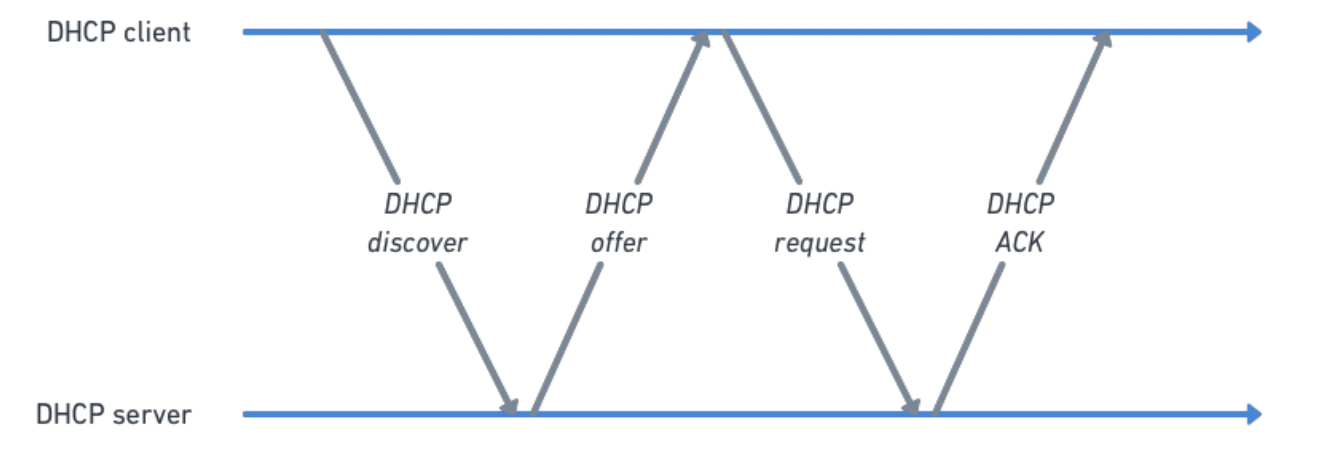
\includegraphics[width=\linewidth]{dhcp}
\end{subfigure}
\hfill
\begin{subfigure}[h]{0.6\linewidth}
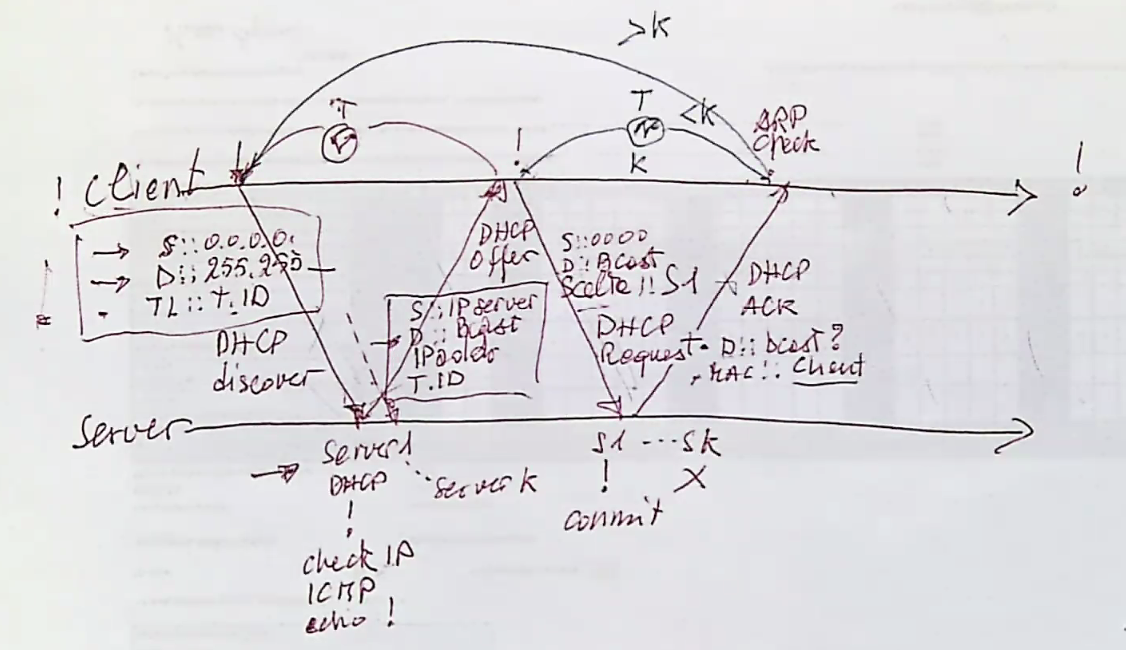
\includegraphics[width=\linewidth]{dhcp2}
\end{subfigure}%
\end{figure}

\section*{ICMP | Internet Control Message Protocol}
E' un protocollo utilizzato per diagnosticare errori in cui un terminale all'interno di un sistema può incorrere. Le principali funzionalità sono: rilevare errori ,rilevare congestione nodi, verificare raggiungibilità nodi, notificare cambio percorso per raggiungere host fornire subnet mask della sottorete e misurare prestazioni dei link. Il formato dei pacchetti ICMP è il seguente:
\begin{center}
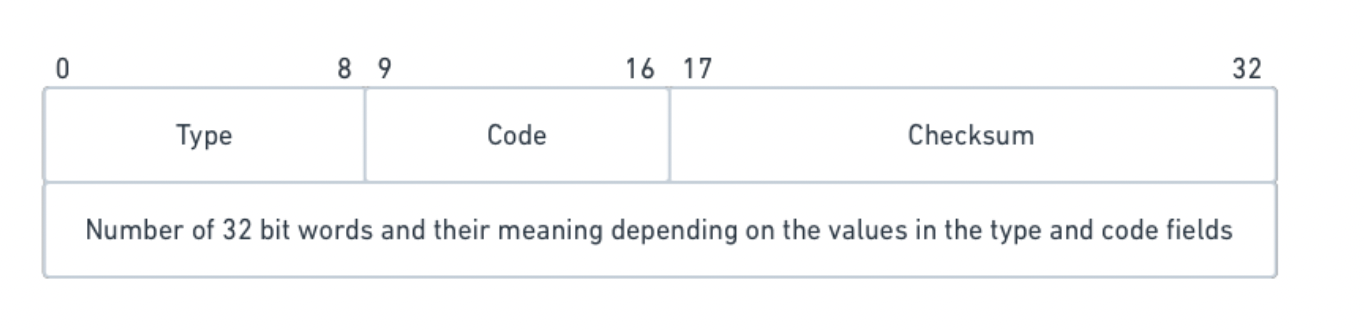
\includegraphics[scale=0.5]{icmp}
\end{center}
Il campo type va ad indicare il tipo di controllo che si vuole effettuare (destination unreachable, time exceeded, parameters error). Il campo code va a complementare il messaggio di informazioni aggiuntive, ad esempio il motivo.

\section*{Routing o Instradamento}
I router, svolgono operazioni di controllo con il protocollo ICMP, e di forwarding (passaggio da una coda di entrata ad una coda di uscita). L'operazione di forwarding è svolta attraverso l'impiego di una tabella di instradamento.\\
La tabella di forwarding, o lookup table è una tabella che associa indirizzi IP di $n$ hosts, e le varie porte di uscite del router su cui instradare il messaggio.\\
La lookup table è popolata dal \emph{router}, attraverso un processo chiamato \textbf{routing}.
A livello 2 viene chiamata forwarding table, mentre a livello 3 è chiamata routing table, rappresenta l'intersezione tra il piano dati ed il piano di controllo
\begin{center}
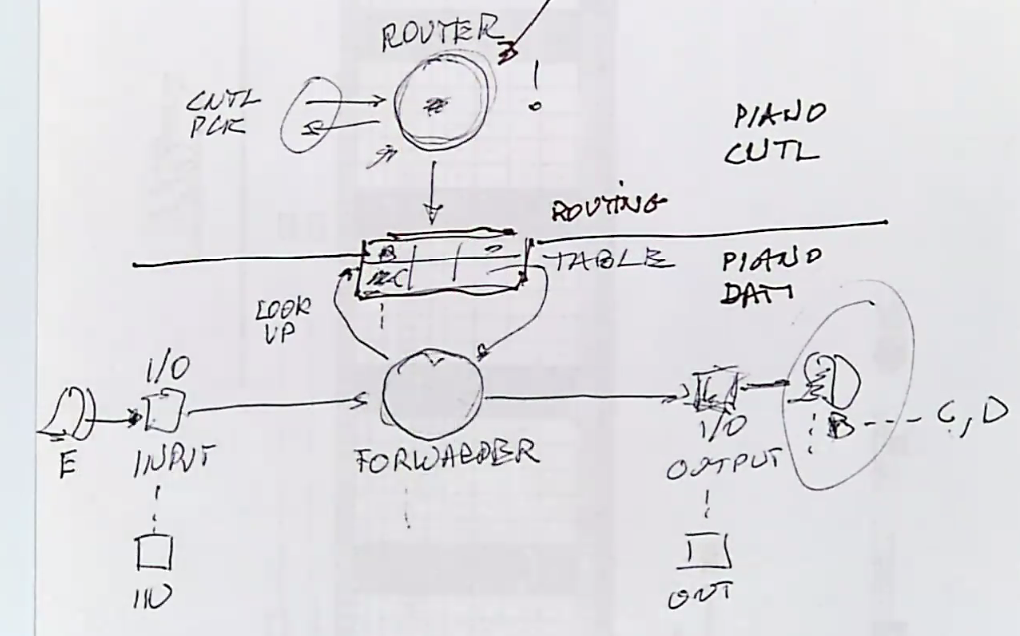
\includegraphics[scale=0.5]{forwarder}
\end{center}
La tabella di instradamento è complementata con una tabella di distanza, chiamata \emph{distance vector}
\subsection*{1 - Distance Vector}
Il distance vector è una tabella che contiene il costo di ogni percorso per raggiungere gli altri host. In particolare vengono salvati i costi dei link, ovvero il numero di hop. I router scambiano periodicamente informazioni riguardo alle proprie tabelle per tenerle aggiornate attraverso un processo chiamato triggered update (impostato) per avere sempre percorsi minimi. La struttura dati utilizzata per memorizzate i distance vector è la tabella di adiacenza
\begin{center}
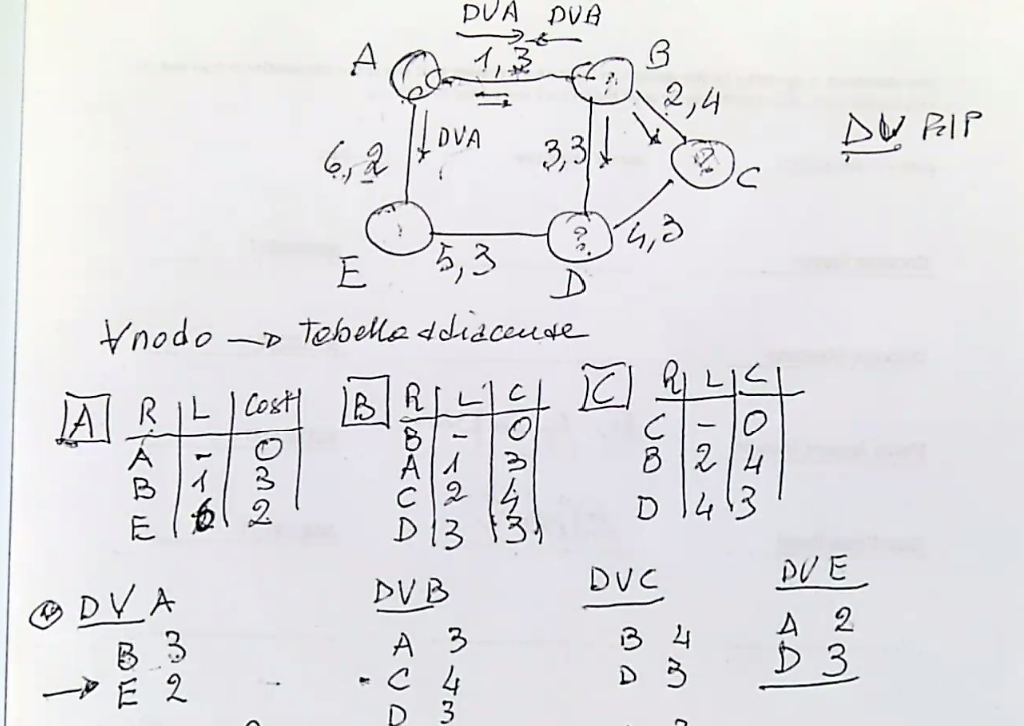
\includegraphics[scale=0.5]{dvector}
\end{center}
\subsection*{Bouncing effect e trigger update}
Il bouncing effect è il caso in cui un collegamento si guasta, il router più vicino se ne accorge subito e nella sua tabella mette $\infty$ al costo per i nodi aldilà di quel collegamento. Poi però un altro router gli invia la sua tabella, dove c'è ancora l'informazione per raggiungere quel nodo con il collegamento guasto e siccome il costo sarà minore di $\infty$ il primo router aggiorna la propria tabella erroneamente.\\
Una possibile soluzione è il trigger update, ovvero quando un router modifica la propria tabella a seguito di un imprevisto, invia a tutti l'aggiornamento senza aspettare il timer. Questa soluzione però non elimina del tutto il problema, perchè il pacchetto di trigger update potrebbe non arrivare a destinazione.
\subsection*{Count to infinity}
Sorge tuttavia un altro problema generato dal bouncing effect, ovvero il count-to-infinity.\\
In un collegamento lineare tra A-B-C-D... se si guasta il collegamento tra A e B, B mette costo infinito ma C poi gli dice che può arrivarci passando tramite lui. Questo propagarsi dell'informazione sbagliata porta a stime di distanza (costo) sempre maggiori.\\
Una possibile soluzione a bouncing effect e count-to-infinity è lo split horizon, in cui ogni router propaga sempre $\infty$ come costo di raggiungimento di stazioni indirette che raggiungerebbe tramite la stazione a cui sta inviando l'informazione. Questa soluzione non elimina del tutto il problema, perché i pacchetti possono comunque perdersi.

\subsection*{La soluzione per entrambi i problemi è usare il protocollo RIP} 
Funzionamento:
\begin{itemize}
\item per ogni entry della tabella di instradamento del router esiste un time. Se per 6
tempi di update (circa 30 secondi l'uno) non ho risposta, allora viene messa la entry a infinity
\item si usa trigger update (c'è sempre il problema count-to-infinity)
\item il costo di un link si indica con il numero di hop nell'intervallo 0:15, con 16 = $\infty$
\item update storm (tempesta di update): può capitare che i timer scadano tutti insieme, quindi viene generato tantisimo traffico in rete, perciò ogni nodo genera il proprio update con un ritardo (0 - 5 secondi)
\end{itemize}


\subsection*{Link state routing}
Invece di scambiare i vettori distanza, si scambiano i vettori di stato.\\
Tutti i nodi trasmettono i costi dei link a loro connessi (link state) non solo ai vicini ma in flooding a tutti gli altri. Un nodo diventa quindi indipendente dagli altri perché tutti hanno le informazioni dell'intera rete. Ci sono un sacco di nodi in più nel traffico di rete, ma questo metodo seleziona il percorso più veloce.
Una volta determinata la tipologia della rete, ogni nodo calcola i cammini minimi verso ogni possibile destinazione con l'algoritmo di Dijkstra (Shortest Path First, SPF).\\
I pacchetti sono caratterizzati da:
\begin{itemize}
\item numero di sequenza, in una topologia magliata, lo stesso link state può giungere da nodi diversi. Si ha quindi bisogno di un meccanismo per droppare i link state già ricevuti
\item fattore di aging, usato per eliminare pacchetti che continuano a girare in rete (e accorgersi di eventuali loop). Può capitare che un pacchetto permanga troppo nella rete (TTL)
\end{itemize}
e sono più piccoli dei vettori distanza, perchè contengono le informazioni dei soli nodi vicini, non di tutta la tabella di un router.
Siccome vengono generati $O(n^2)$ messaggi nella rete per costruire le tabelle, si designa un router predefinito (designated router), a cui vengono inviati tutti gli stati e che poi calcolerà i cammini minimi e li manderà in flooding a tutti i suoi nodi ogni periodo di tempo (di solito solo se cambiano).

\subsection*{2 - OSPF | Open Shortest Path First}
È il protocollo di internet definito nell'RFC 2328 che gestisce la gran parte dei problemi di routing con tecnica Link State. Opera:\begin{itemize}
\item negli autonomous system (sistemi autonomi), composti da diverse sottoreti
collegate a un'area zero.
\item tra aree backbone (aree zero), aree più alte a livello gerarchico, che possono essere composte sia da router che da sottoreti. Nell'area zero ci sono speciali routers, chiamati AS boundary routers, che fungono da gateway tra la sottorete degli host e la internet backbone (dorsale internet), mentre i router che collegano le sottoreti all'area zero si chiamano border routers. Nell'aree zero, per evitare problemi relativi al flooding, vi è un \textbf{designated router} che concentra su di se gli aggiornamenti per le tabelle di routing e distribuisce poi le informazioni complete ai nodi vicini (vedi link state)
\end{itemize}
\begin{center}
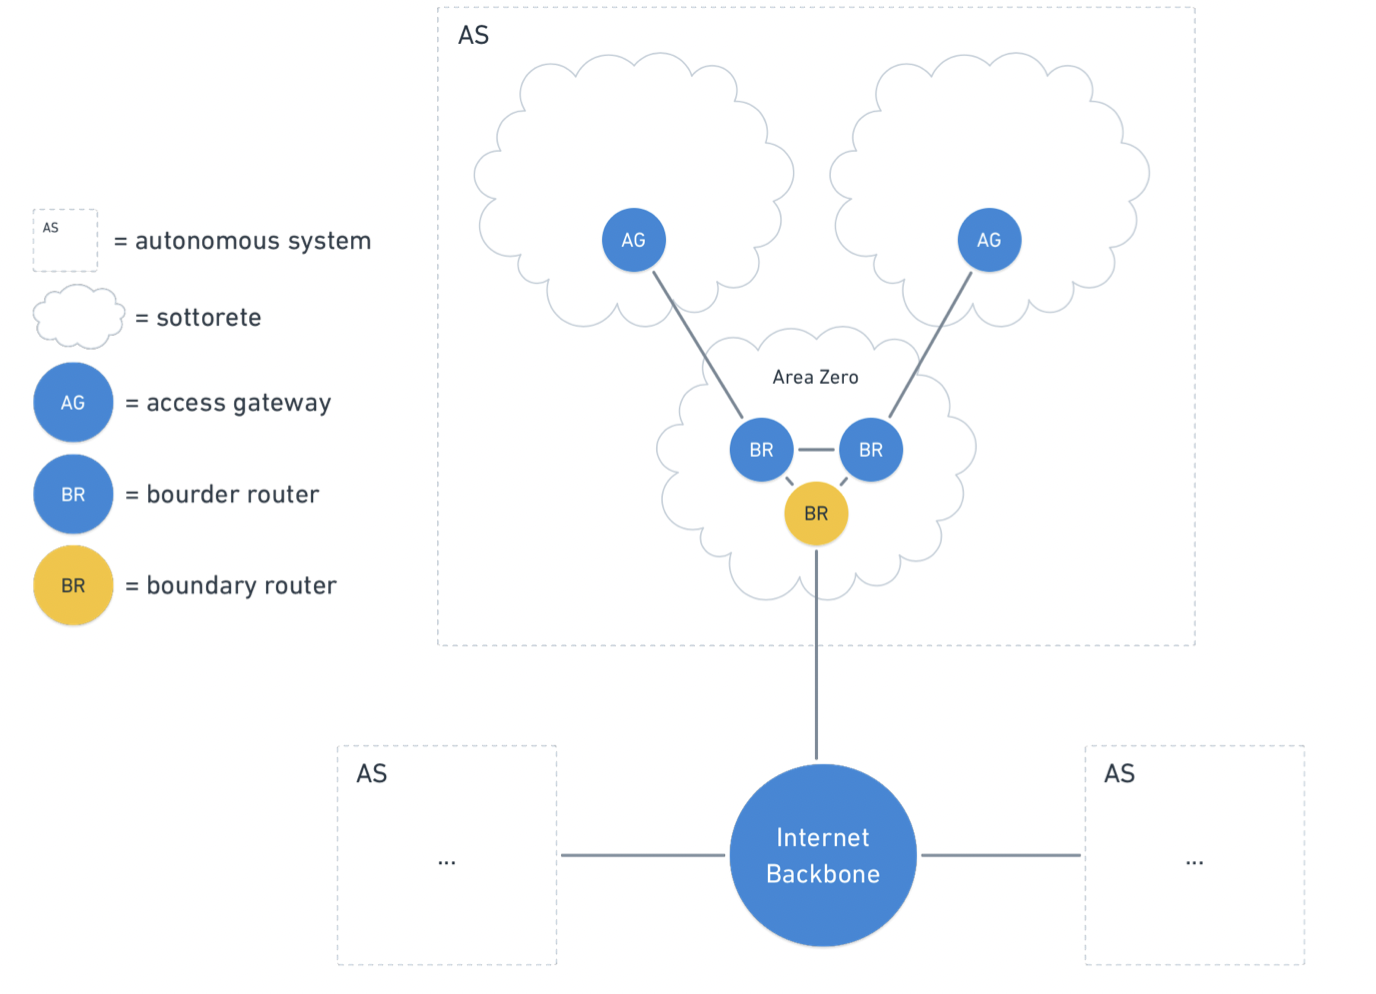
\includegraphics[scale=0.5]{route}
\end{center}
Le operazioni che vengono svolte durante l'OSPF sono:
\begin{itemize}
\item Hello, usato da un router per scoprire nuove reti/router adiacenti, scoprendo così il costo di un link
\item Link State Update, inviato dal designated router ad intervalli periodici (o quando necessario, tipo cambiamento costi link, etc) che porta con se le informazioni riguardanti le tabelle di routing, da far propagare agli altri router
\item Link State ACK, ogni router valida un Link State Update con questo messaggio 
\item Database Description, viene usato per informare il ricevente del messaggio se è disponibile o meno un aggiornamento
\item Link State Request, viene usato per richiedere un Link State Update da ogni router adiacente
\end{itemize}

\subsection*{3 - BGP | Border Gateway Protocol}
Un protocollo a livello 3, che tuttavia interagisci col livello 2 (TCP) attraverso la porta 179. Opera sfruttando un approccio simile al Distance Vector, che tuttavia viene modificato: al posto di mantenere solamente la destinazione, esplicita anche il l'intero cammino. 
Qualora un collegamento viene interrotto, conoscendo l'intera topografia del cammino siamo in grado di scartare il cammino, scegliendone uno alternativo.
\begin{center}
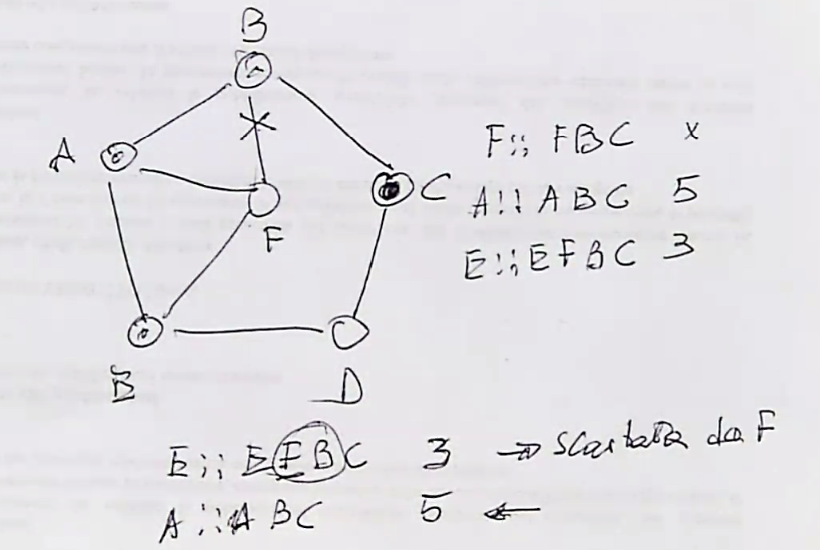
\includegraphics[scale=0.5]{bgp}
\end{center}
\footnotesize{La sezione dei messaggi è ignorata}

\subsection*{MPLS | Multi Protocol Label Switching}
\begin{center}
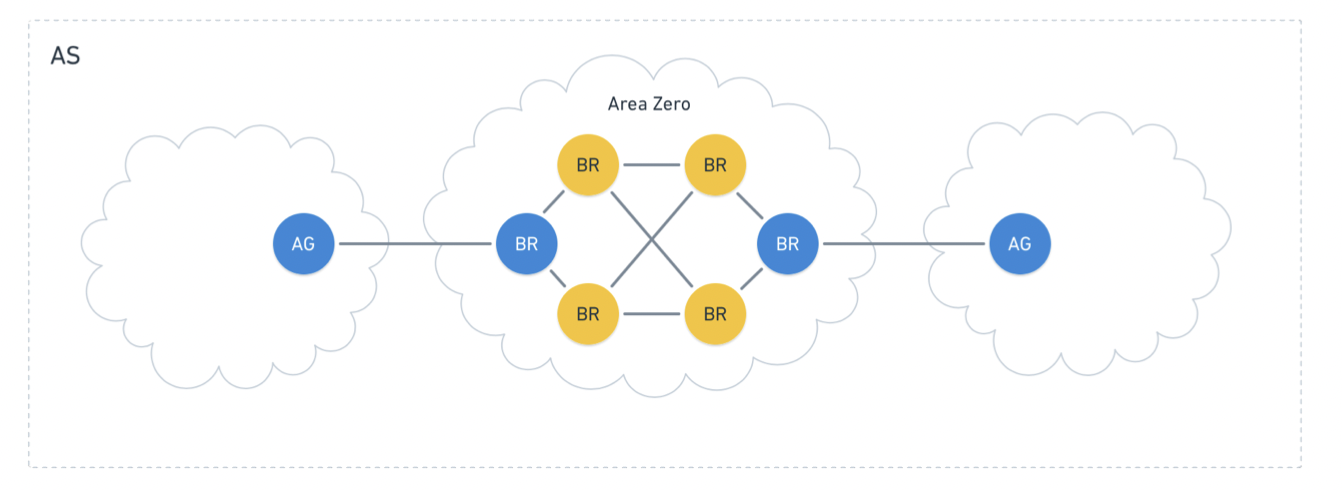
\includegraphics[scale=0.5]{mpls}
\end{center}
Questo protocollo va a sostituire l'OSPF, lo switching viene effettuato introducendo delle labels (etichette), alla quale vengono anche incorporate identificatori di priorità. I pacchetti in entrata non vengono modificati, la tupla IP ed il Payload sono mantenuti, ma vengono incorporati con un involucro utilizzato per svolgere l'operazione di tunneling\\
Una visione ad alto livello:
\begin{center}
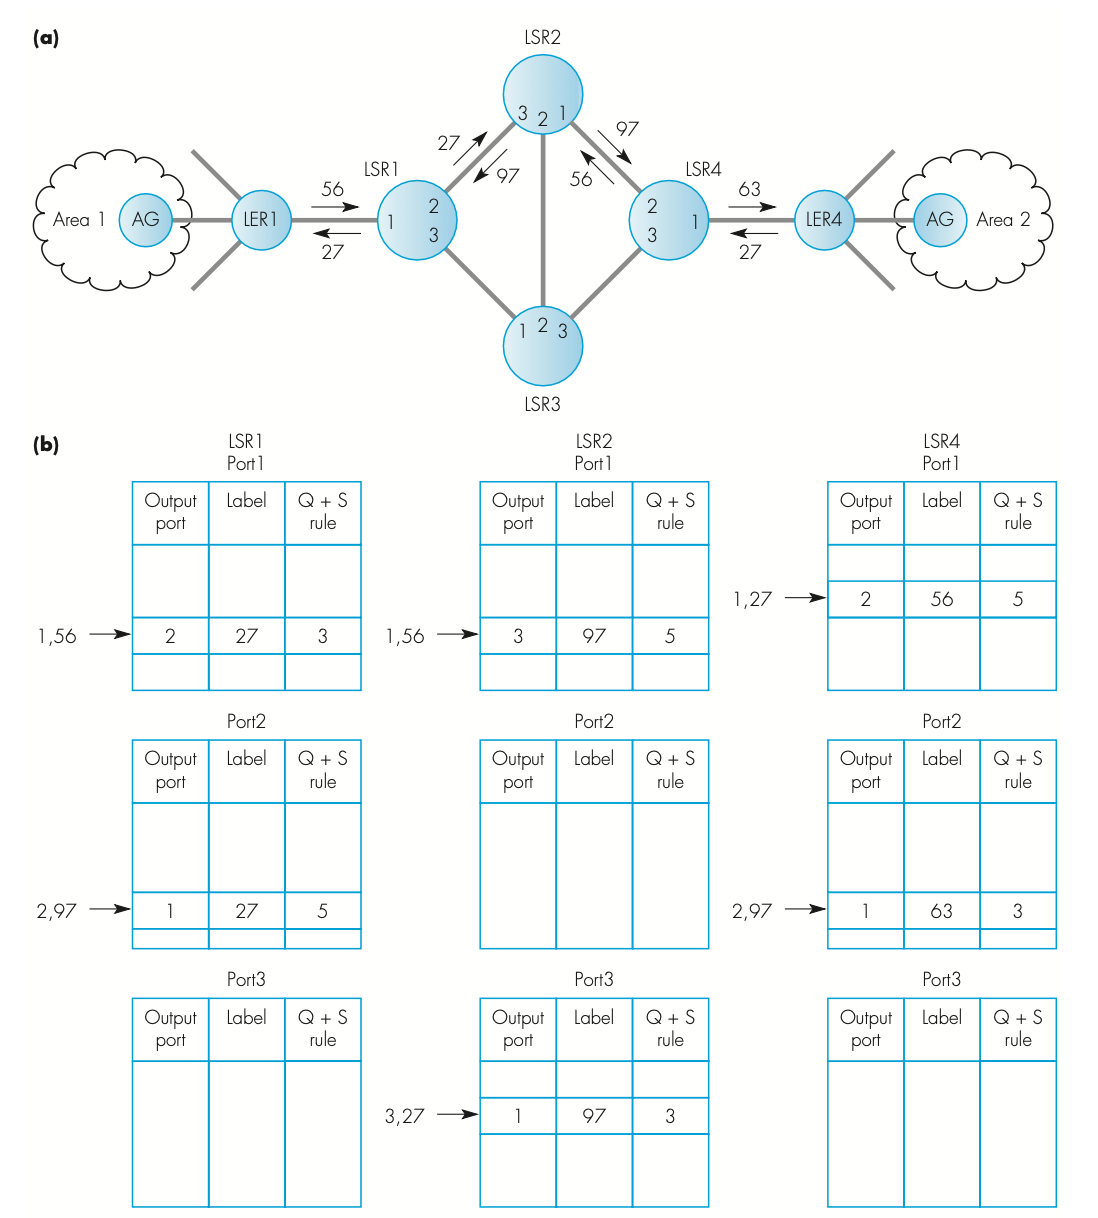
\includegraphics[scale=0.5]{etichettatore}\\
\emph{Il pacchetto in entrata in LER1 con etichetta 1, diventa l = 56 entra in LSR1 da porta 1 ed esce da porta 2 come indicato nella LSR table}\\
\emph{quando esce da $LSR1_2$, l = 27, entra in LSR2} ...  
\end{center}
Il componente LER1 (label edge router) associa un header che viene utilizzato dagli altri LSR (label switch router) per inoltrare i package. Gli LSR mantengono una label switching table. \\
\textbf{La label switching table} contiene entries per ogni porta in entrata, ed ogni porta in uscita, così come labels da assegnare. Le labels cambiano ogni volta che il pacchetto passa per un LSR.
\subsubsection*{Label edge router}
\begin{center}
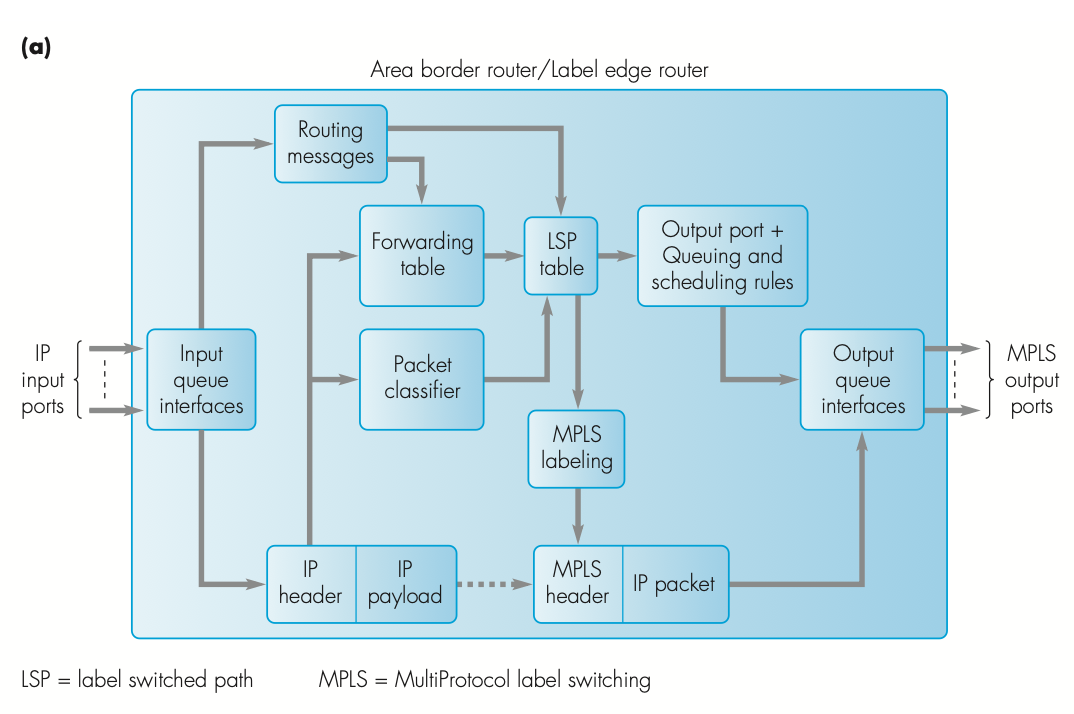
\includegraphics[scale=0.5]{et1}\
\end{center}
I pacchetti non vengono inoltrati secondo l'IP Header (passando per la forwarding table), ma secondo un MPLS header, che viene integrato all'IP packet. Il label edge router provvede ad aggiungere/rimuovere l'intestazione MPLS dalla testa dei pacchetti IP, poiché MPLS ha senso solo ad ogni hop. E' funzionale solo a velocizzare il processo di switching ma è ininfluente a livello di routing.
\begin{center}
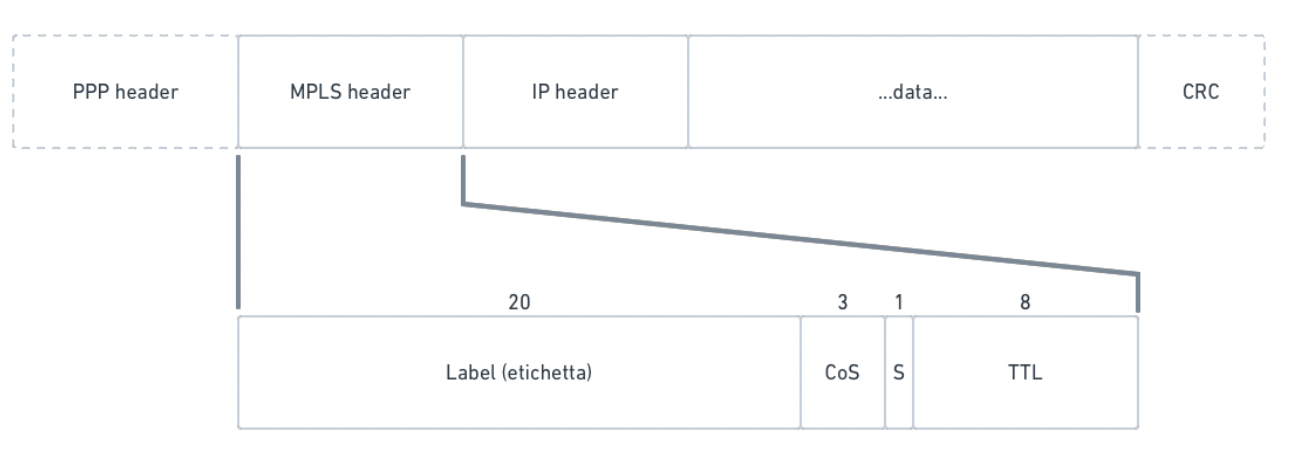
\includegraphics[scale=0.5]{newlabel}\\ 
\end{center}
- Il campo COS va ad identificare la regola di scheduling\\
- Il campo label identifica la politica per il singolo hop, così come l'identificatore per la porta d'uscita.\\
\subsection{Gestione delle congestioni | RED}
Il Random early detection (o RED), è un meccanismo utilizzato per prevedere e prevenire l'insorgere della congestione nelle reti. Ogni router viene programmato perché tenga sotto controllo le proprie code, ma quando si accorge che una congestione è imminente viene inoltrato un segnale alla sorgente della congestione, che elimina anticipatamente dei pacchetti. 

\subsection*{review}
Code di priorità -> come gestisco l'instradamento nelle code? -> lookup type of service

\section*{IPv6}
Nato per sostituire IPv4 e la mancanza di indirizzi, aggiunge nuove funzionalità.
\begin{center}
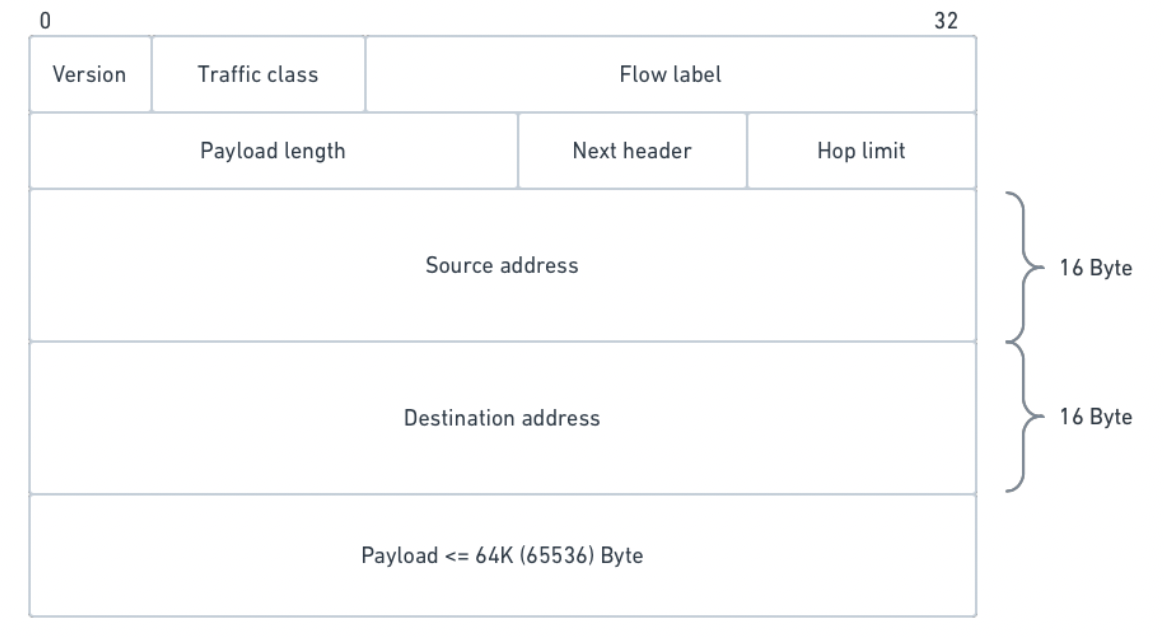
\includegraphics[scale=0.5]{ipv6}
\emph{4 parole da 32 bits}
\end{center}
Una caratteristica particolare di IPv6 è l'interoperabilità con i protocolli IPv4, questo viene fatto inglobando l'indirizzo a 32 bit all'interno dell'indirizzo IPv6. (vengono utilizzati i bits a destra)
\subsection*{8 byte di parametri}
\begin{itemize}
\item version (4 bit), indica la versione del datagramma IP: per IPv6 è settato a 6 
\item traffic class (8 bit) (corrisponde a type of service), si traduce come "classe di traffico", successore di ToS, classifica il pacchetto favorendo regole di routing e lo smistamento assegnando una classe di priorità, rispetto ad altri pacchetti provenienti dalla stessa sorgente
\item flow label (20 bit), usata dal mittente per etichettare una sequenza di pacchetti come se fossero nello stesso flusso. Aiuta nella gestione del QoS (Quality of Service), nel controllo di flusso, anche se ancora in fase sperimentale. Per best-effort è settato a 0 .
\item payload length (16 bit), è la dimensione del payload, ovvero il numero di byte di tutto ciò che viene dopo l'header. Eventuali estensioni dell'header sono considerate payload. Max a 64 KB, minimo a 536 B (perchè 536 B + 40 B di header = 576 B, minimo per far si che il pacchetto non venga frammentato) 
\item next header (8 bit), va a puntare al prossimo header, può puntare\\
- all'header del livello superiore (ad esempio TCP)\\
- ad un ulteriore next header, attraverso un processo chiamato \emph{header extension}, che può a sua volta puntare ad un'altro next header (lista concatenata). La sequenza deve tuttavia terminare con TCP
\item hop limit (8 bit), è il limite di salti consentito, praticamente è il TTL per IPv6, con default a 256
\end{itemize}
\subsection*{32 Byte per indirizzi}
\begin{itemize}
\item source address, 16 Byte per indirizzo sorgente 
\item destination address, 16 Byte per indirizzo destinazione
\end{itemize}
\subsection*{Formato di un indirizzo IPv6}
Un indirizzo IPv6 è rappresentato con 8 blocchi da 16 bit divisi da $:$. Questi blocchi per comodità vengono scritti in esadecimale, blocchi contigui di $0$ possono essere omessi e sostituiti con $::$.
\begin{center}
$16bit:16bit:16bit:16bit:16bit:16bit:16bit:16bit$\\
$BA98 : 7654 : 3210 : 0000 : 0000 : 0000 : 0089$\\
$BA98 : 7654 : 3210 :: 0089$
\end{center}
Per agevolare l'operazione di instradamento dei pacchetti IPv6, vengono definiti una serie di $Tiers$, in base alla grandezza del servizio:
\begin{itemize}
\item Tier1: organizzazioni a livello continentale, rappresentati da $registry, TLA$
\item Tier2: organizzazioni a livello nazionale, rappresentati da $NLA$
\item Tier3: organizzazione a livello locale, rappresentato da $SLA$
\end{itemize}
\begin{center}
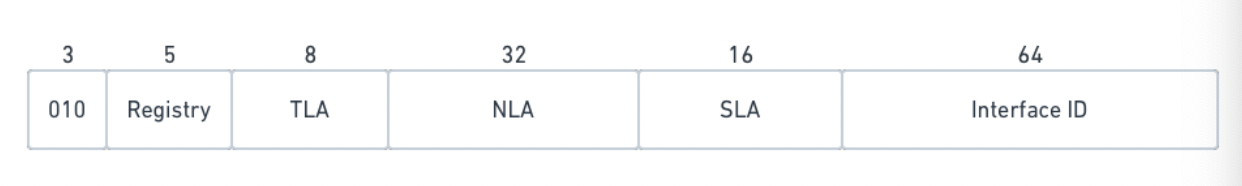
\includegraphics[scale=0.5]{routingtable}
\end{center}
$010$ rappresenta un prefisso che indica la comunicazione punto punto \\$registry$ il continente, $TLA$ la nazione, $NLA$ la zona intra-nazionale, $SLA$ la zona locale.\\
L'interface ID è suddiviso in 16 bit per la sottorete, e 48 bit corrispondente all'indirizzo MAC dell'host.\\\\
\section*{Livello 4 "Trasporto"}
Il come inviare i messaggi è risolto nei livelli 1-3. Ora vediamo come mettere in comunicazione applicazioni da un host A a un host B (collegamento end-to-end). \\
A livello 4 si spediscono e si ricevono segmenti. In particolare ci interessiamo del protocollo TCP, affidabile (e UDP, non affidabile, UDP è più semplice). I principali temi che vogliamo trattare sono l'affidabilità, e l'indirizzamento.\\\\
Consideriamo un client ed un web server, come fanno i due dispositivi a distinguere i segmenti da un dispotivi all'altro? Ci troviamo quindi davanti ad un problema di smistamento, sia mentre effetuiamo un'operazione di request, sia mentre riceviamo una answer.
\begin{center}
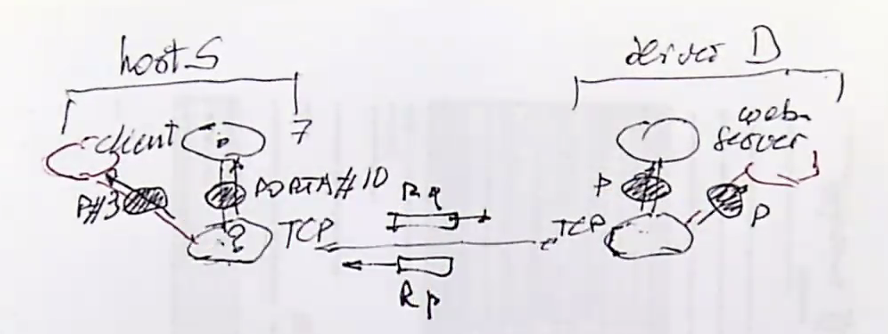
\includegraphics[scale=0.5]{t1}
\end{center}
A livello 3 abbiamo il protocol selector, basato su ARP/RARP, a livello 4 invece, risolviamo il problema attraverso l'impiego di uno strumento chiamato porta, o socket. In particolare per gestire il trasferimento di segmenti a livello 4:
\begin{itemize}
\item associamo una porta ad un nome simbolico di servizio sorgente, che può essere un sito web, posta elettronica, etc., il valore è chiamato $P_{ID}Sorgente$ è fornito dal socket
\item associamo una porta ad un nome simbolico di servizio destinatario, il valore è chiamato $P_{ID}Destinazione$ ed è definito a partire dalle well known ports.
\end{itemize}
La coppia \begin{center}
$<P_{ID}Sorgente,P_{ID}Destinatario>$ \end{center}determina in maniera univoca la richiesta, che viene gestita dalla porta in destinazione secondo la politica definita. \\
In totale le porte possibili sono $2^{16}$:
\begin{itemize}
\item dalla 0 alla 1023 sono le well known ports, che sono associate a servizi di standard (mail, web, etc.)
\item dalla 1024 alla 49151 sono associate a servizi famosi
\item le porte successive sono lasciate libere
\end{itemize}
Questo tuttavia non basta è intuibile diversi servizi abbiamo più porte dello stesso valore, ad esempio Google, Facebook, Microsoft hanno rispettivamente una porta $80$ da gestire. Entrano quindi in gioco gli indirizzi IP dei singoli servizi. Una singola request diventa quindi:
\begin{center}
$<P_{ID}Sorgente,P_{ID}Destinatario, IP_D, IP_S>$
\end{center}
Il valore di $IP_D$ è ricavato dal DNS, che vedremo più avanti, e intuitivamente il valore di $IP_S$ è ricavato in locale.
\subsection*{TCP | web server}
Consideriamo un web server che riceve $k$ requests, come fa a gestirle e restituire $k$ replies? \\In genere un web server gestisce più \emph{forks} per gestire in parallelo più requests, tuttavia queste non tutte possono avere la stessa porta altrimenti verrebbero mischiate tutte le requests. \\\\Assegniamo quindi una porta $(x, ... y)$ ad ogni singolo thread $(1, ... k)$, ed impieghiamo quindi una tabella che lavora similmente al NAT, che le indicizza, e smista le requests.
\begin{center}
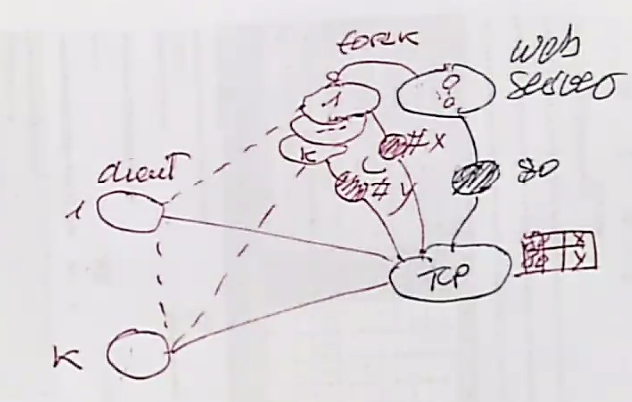
\includegraphics[scale=0.5]{t2}
\end{center}
In questo modo se un $client_1$ genera una request, il traffico gestito da TCP è smistato al $fork_{client_1}$ del web server.
\subsection*{Overview di TCP}
TCP è il primo protocollo che vediamo che è orientato alla connessione, ovvero la capacità di associare univocamente un processo lato client con un processo lato server. 
\begin{center}
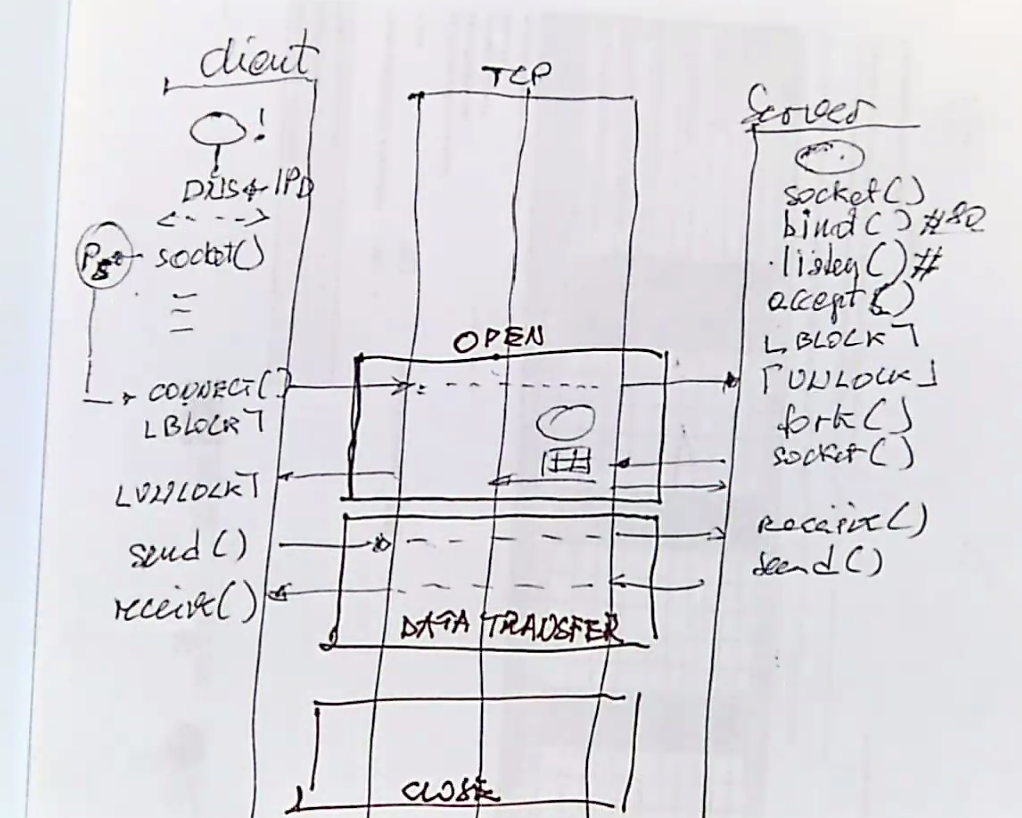
\includegraphics[scale=0.5]{t3}
\end{center}
Le connessione possono quindi trovarsi in 3 fasi, open, data transfer, e close.
\subsection*{Header di TCP}
\begin{center}
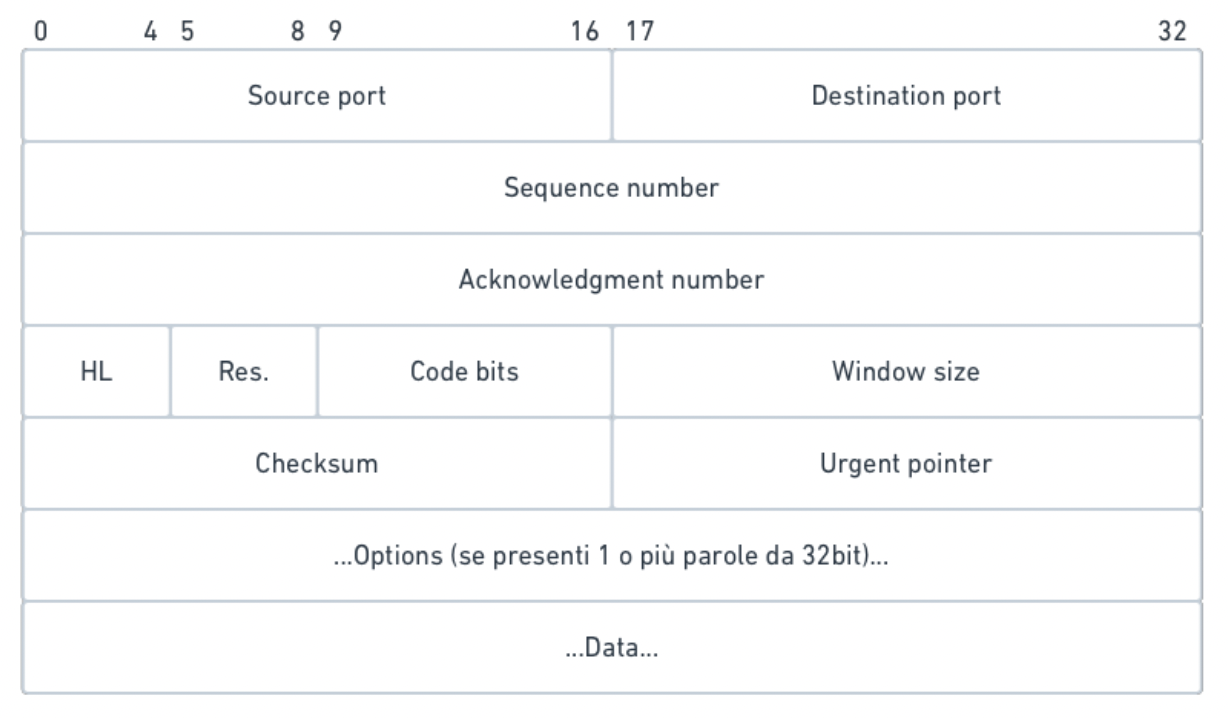
\includegraphics[scale=0.5]{t4}
\end{center}
\begin{itemize}

\item source port (16 bit), identifica il numero di porta sull'host mittente associato alla connessione TCP
\item destination port (16 bit), identifica il numero di porta sull'host destinatario associato alla connessione TCP
\item sequence number (32 bit), numero del segmento del dato da trasferire. Numera i Byte, perchè TCP considera payload come stringhe di Byte. È puntatore al primo Byte nel campo dati
\item acknowledgment number (32 bit), ha significato solo se il campo ACK è impostato a 1. È usato solo dalla destinazione, che per convenzione indica il numero del segmento che si aspetta di ricevere (quindi successivo all'ultimo convalidato/arrivato).
\item HL (Header Length o Data Offset), numero di parole da 32 bit presenti nel campo Options (header ha lunghezza variabile)
\item Res. (Reserved) (4 bit), bit non utilizzati e predisposti per sviluppi futuri del protocollo
\item code bits (6 bit), maschera di 6 bit che identifica il tipo di segmento. Più bit possono essere settati a 1, aggiungendo più informazioni in un singolo segmento. I possibili valori sono:\\
- SYN: stabilisce una connessione\\
- ACK: conferma della validità del campo\\
- FIN: chiude la connessione\\
- PHS: invio dei dati alla ricezione di questo segmento URG: urgente\\
- RST: rifiuta una richiesta di connessione o ripristina i valori iniziali del numero\\
di sequenza
\item window size (16 bit), anche "Advertise Window", è la larghezza della finestra per spedire i frammenti. La dimensione è decisa a priori, prima di iniziare la comunicazione, e scelta in base alla dimensione massima di trasferimento del canale in uso e del buffer lato destinazione. Si usa per evitare la frammentazione 
\item checksum, contrariamente al checksum del pacchetto IP (che riguardava solo l'header), questo riguarda tutto il segmento, cioè header + payload. Inoltre alcuni campi del pacchetto IP sono inclusi nella generazione di questo checksum e formano il cosiddetto \textbf{TCP pseudo header}
\item urgent pointer (16 bit), denota il numero di Byte nel campo dati che deve essere subito consegnato all'applicazione che sta comunicando. Ha significato solo se il code bit "URG" è settato a 1 e indica lo scostamento in Byte a partire dal numero di sequenza dei dati urgenti del flusso
\item options, usato per descrivere, ad esempio, la dimensione massima di un segmento (MSS - Maximum Segment Size). Se non specificata viene scelta di default a 536 Byte (poiché sommando header TCP e IP ottengo i famosi 576 Byte)
\item payload, rappresenta i dati da trasmettere
\end{itemize}

\subsection*{Pseudoheader di TCP}
Lo pseudoheader di TCP è creato a partire da\begin{center}
 $<P_{ID}Sorgente,P_{ID}Destinatario, PSEC, SL>$\end{center} è utilizzato per calcolare il checksum. Lo pseudo header non viene spedito, ma viene costruito localmente da ogni macchina.
 
\subsection*{Apertura di una connessione}
A connessione chiusa:
\begin{center}
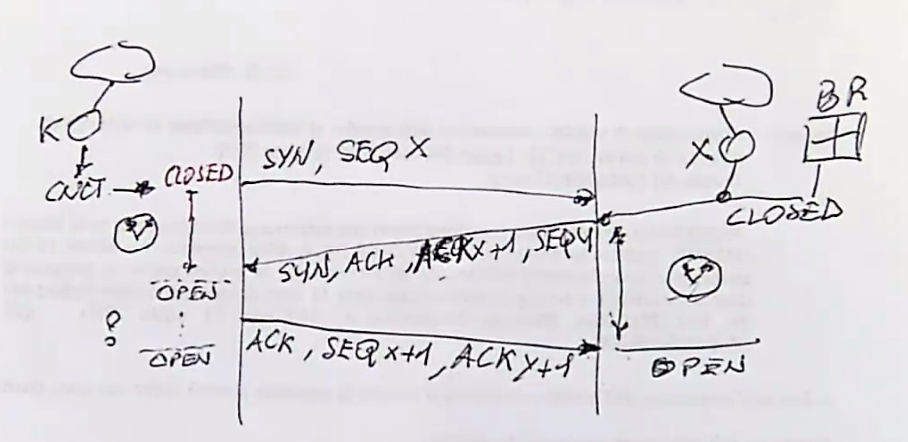
\includegraphics[scale=0.5]{t5}
\end{center}
\begin{itemize}
\item il client manda un segmento con bit $SYN_1$, e come numero di sequenza un valore $x$.
Il valore $x$ chiamato ISN, o Initial Sequence Number, è un valore pseudorandom, generato dal client e utilizzato in futuro come riferimento
\item il server ha già allocato un buffer di ricezione (BR) per la gestione di request, e risponde con \begin{center}
$SYN_1, ACK, ACK$ $x+1$, $SEQ$ $Y$ 
\end{center}
Per convenzione viene convalidato anche il pacchetto successivo, attraverso l'$ACK_{x+1}$, l'ACK è necessario TCP ogni messaggio deve essere validato.
La $SEQ$ $Y$ è generato da server, e viene poi utilizzato come riferimento per tutti i successivi messaggi
\item Il client risponde con \begin{center}

$ACK, SEQ x+1$, $ACK$ $y+1$\\
\end{center}
La connessione è quindi stabilita
\end{itemize}

\subsection*{Data transfer}
A connessione aperta:
\begin{center}
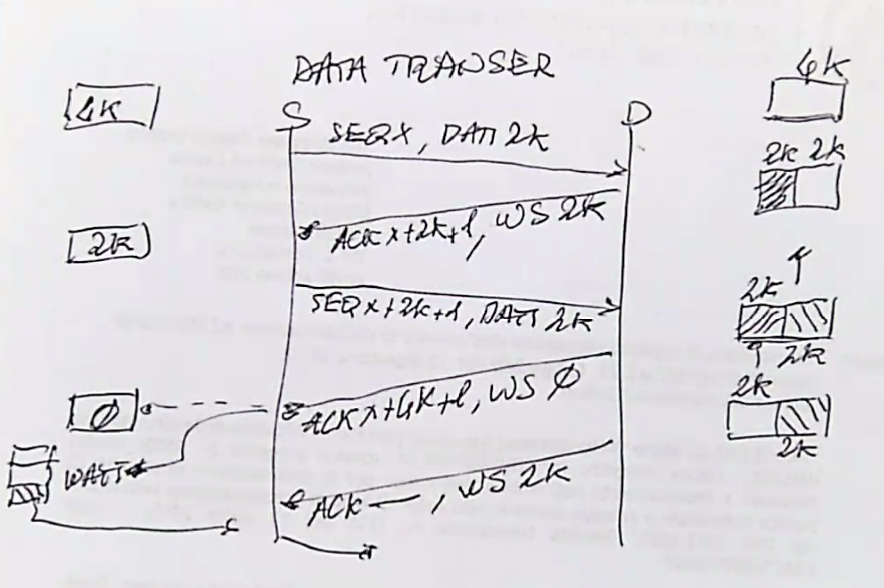
\includegraphics[scale=0.5]{t6}
\end{center}
Il campo Window Size nel segmento TCP serve a regolare quanti Byte inviare/poter ricevere.\\
Il destinatario fa sapere quanti Byte può ricevere (se ha buffer di ricezione vuoto saranno uguali a quanto è grande il buffer). Man mano che il mittente invia blocchi di $N$ Byte, il destinatario occuperà il buffer con quei dati, e risponderà indicando la nuova dimensione (diminuita) del buffer di ricezione, cosicchè il mittente sappia quanti Byte mandare al massimo nel prossimo segmento che dovrà inviare.\\
Se il server non può più ricevere, comunica al client che la sua window size è 0, e il client si metterà in attesa di una nuova comunicazione del server con window size > 0.
In caso di perdita dell'ACK che aggiorna dal server al client la window size disponibile (window update) ci sono due strategie di recovery:\begin{itemize}
\item Persistent timer (per la salvaguardia del client): ogni connessione è dotato di un timer chiamato persist timer, ogni qualvolta venga ricevuto un segmento con $window size = 0$ il persist timer è avviato (solitamente per 60 secondi). Se non viene ricevuto nessun aggiornamento viene generato un \emph{window probe} che richiede nuovamente al server l'ACK perduto. Se dopo $n$ probes non viene ricevuta nessuna risposta, il client chiude la connessione
\item Keep Alive Timer (per la salvaguardia del server): il server ha un timer locale (solitamente settato a 2 ore), che allo scadere genera un \emph{keep alive probe} per verificare se il client è ancora attivo. 
Se dopo $n$ probes non viene ricevuta nessuna risposta, il server chiude la connessione
\end{itemize}

\subsubsection*{Selective repeat | timer di ritrasmissione}
Lo schema di comunicazione è a modello cumulativo, qualora un ACK non arriva, viene validato l'ultima sequenza corretta, in questo esempio è $ACK x+2001$ e dopo $n$ tempo viene reinoltrato il messaggio droppato
\begin{center}
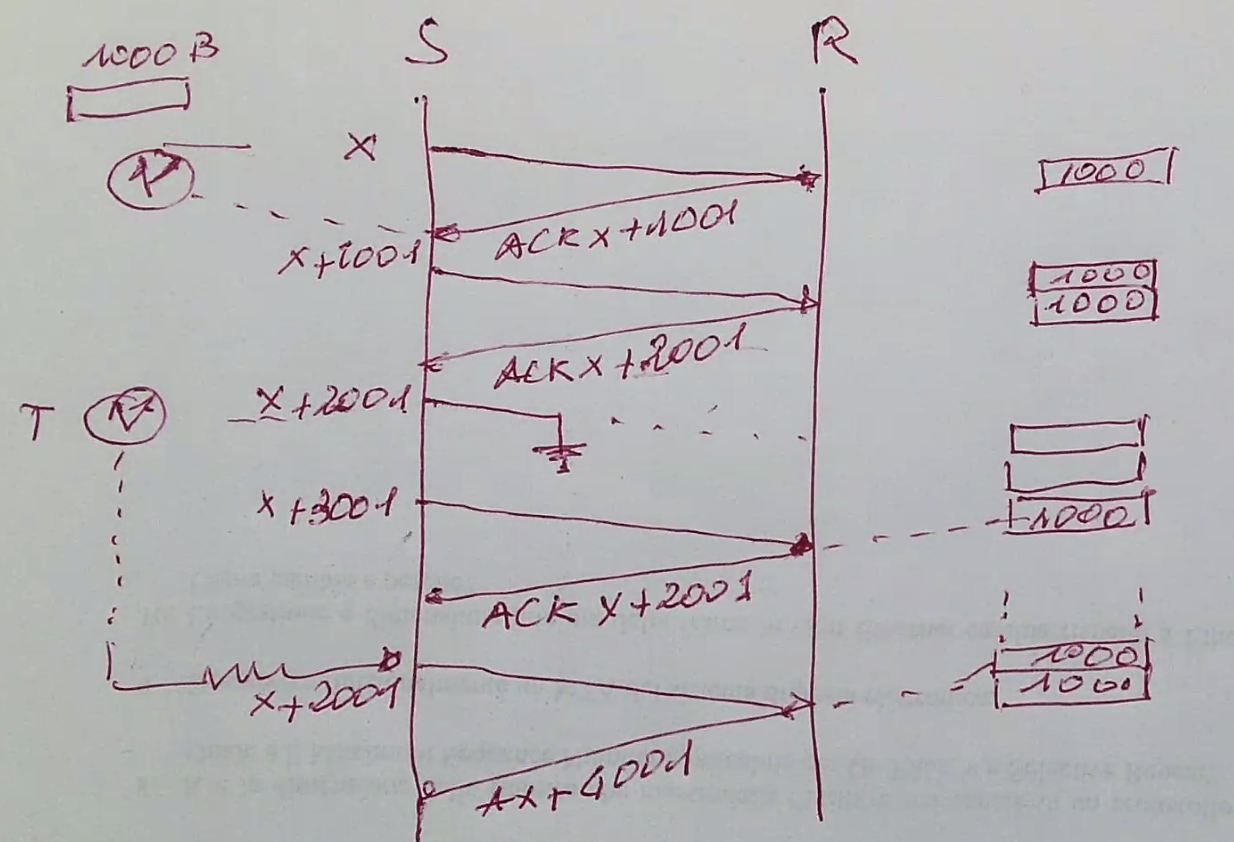
\includegraphics[scale=0.5]{t7}
\end{center}
Dobbiamo tuttavia fare due considerazione:\begin{itemize}
\item a lato ricevente stiamo lavorando secondo un modello selective repeat (e non go-back-n), quando non viene ricevuto un pacchetto, non dobbiamo inoltrare tutti i pacchetti a partire dal droppato, ma solo quello droppato
\item il timer di trasmissione deve essere ben dimensionato, in base al tempo di trasmissione. \\\emph{ma come dimensioniamo il timer?} Non possiamo utilizzare il RTT (round trip time), in quanto può essere variabile, inoltre a livello 4 dobbiamo considerare i componenti di rete (router, switches etc.)\\ Vengono fatte delle stime, ed è poi sovradimensionato il timer.
\end{itemize}
\subsubsection*{Problematiche sul timer}
\begin{itemize}
\item grandezza del timer: Siccome siamo su internet, a quanto si dimensiona il timer RTO? Se troppo grande spreco tempo! RTO dipende dall'RTT, che può variare durante una connessione, quindi dovràà variare anche RTO. Inizialmente si parte con un valore di RTO relativamente elevato:
\item fast retransmit: per evitare che una connessione si blocchi perché un timer è stato sovradimensionato o perché al server è arrivato un segmento non in ordine. Ogni volta che al server arriva un segmento non in ordine (ne manca uno in mezzo) manda un ACK specifico avvertendo che si è "fuori sequenza". Quando poi al server arriverà/arriveranno i segmenti mancanti manderà un ACK avvertendo che tutto è ritornato ok (ACK cumulativo). 
Anticipa il reset del timer di ritrasmissione dopo aver ricevuto $n$ ack fuori sequenza. In particolare in questo esempio dopo 3 ACK fuori sequenza il timer è resettato, e il client reinvia il segmento.
\begin{center}
\includegraphics[scale=0.5]{t8}
\end{center}
\end{itemize}
\subsection*{Ottimizzazione del data transfer}
Consideriamo un utente che deve inviare una bassa quantità di dati alla volta, per esempio inoltrando un carattere alla volta, il traffico risulta fortemente oneroso in quanto ogni segmento inviato genera un ACK di risposta. 
\subsubsection*{Delayed acknowledgements}
Delayed acknowledgements consiste nel far attendere il server un tempo prefissato (200ms) dopo la ricezione di un segmento, e aspettare eventuali altri dati, così da inviare un unico ACK complessivo e ridurre quindi il numero di segmenti in rete. In caso di applicazioni utente che devono essere responsive (vedi telnet, server di echo), si potrebbe creare un delay inaccettabile per l'utente.
\subsubsection*{Algoritmo di Nagle}
L'algoritmo di Nagle cerca di raggirare il problema, in particolare  è una versione modificata del delayed acknowledgements, per cui un'entità TCP può avere un solo "segmento piccolo" alla volta, in attesa di ACK. In questo modo il client invia un segmento piccolo e mentre aspetta la ricezione dell'ACK del server, il suo buffer di invio si riempie, così che quando sarà nuovamente possibile inviare (alla ricezione dell'ACK spedito dal server) riesca ad inviare più informazioni in un unico segmento. In particolare viene creato anche un buffer a lato server, e solo qualora una data soglia di volume di dati per creare un segmento di risposta è raggiunto, esso viene inviato attraverso una tecnica chiamata piggybacking. 
\subsubsection*{Algoritmo di Clark}
algoritmo di clark, cerca di diminuire al minimo i window update, consiste nel compattare i window update lato server, cioè ritardare la spedizione del window update (dopo il window update 0) finchè il buffer di ricezione del server abbia raggiunto la Maximum Segment Size oppure se raggiunge la metà della memoria disponibile. In questo modo il server non informerà mai il client se la dimensione della finestra è piccola, e quest'ultimo non invierà mai segmenti contenenti una quantità ridotta di dati.

\subsection*{Dimensionamento della finestra di trasmissione | congestion window}
Dimensionare la finestra di trasmissione (o window congestion) che deve essere:
\begin{center}
$W_t/c = MIN(NET,BUF | RIC)$
\end{center}
TCP deve essere in grado di intuire lo stato di saturazione della rete, il minimo tra il la grandezza del buffer di ricezione, e dello stato della rete.  Siccome TCP può avere più connessioni simultanee e non sa la capacità del canale, ma lavora solo sulla grandezza della finestra di invio, concordata con il ricevitore, adotta un approccio cauto.\\
Inizia scegliendo la finestra più piccola possibile, per poi aumentarla fino al limite imposto dal ricevitore. Quando avviene un errore si azzera tutto e si riparte.\\
Nel caso non si verifichino errori (o perdita ACK), TCP divide il trasferimento dati in 2 fasi:
\begin{itemize}
\item Slow start, si trasmettono segmenti piccoli partendo dalla dimensione minima dei segmenti stabilita all'apertura della connessione e con dimensione finestra a 1. Ad ogni ACK ricevuto correttamente la dimensione della finestra raddoppia. Questa fase viene iterata fino a che non si raggiunge la soglia SST (Slow Start Threshold) (pari alla metà della dimensione massima della finestra).
\item  Congestion Avoidance, all'inizio di questa fase la finestra di congestione ha
come dimensione SST. Da questo punto in poi (sempre se non si verificano errori) TCP trasmette finestre aumentandone la dimensione linearmente (aggiungo 1 segmento alla finestra dopo aver ricevuto tutti gli ACK per la scorsa finestra). Raggiunta la soglia massima trasferibile, la dimensione non cambia più. La crescita diventa lineare
\end{itemize}
\begin{center}
\includegraphics[scale=0.5]{t9}
\end{center}
La gestione nel caso di errore è definita all'interno della policy RFC 5681: 
\begin{itemize}
\item viene utilizzato RTO nel caso sia scaduto il timer di trasmissione, in quanto si ipotizza che la rete sia congestionata. Il fast retransmit prevedeva che il client aspettasse 3 ACK "fuori sequenza" prima di reinviare un pacchetto perso. Per il controllo della congestione questo non è considerato un errore grave, in quanto il server ha comunque ricevuto quasi tutti i pacchetti. Però alla ricezione del terzo ACK "fuori sequenza" si imposta un nuovo valore per SST pari all'attuale finestra dimezzata e si modifica comunque la grandezza della finestra di invio portandola al minimo tra l'SST iniziale e quello appena calcolato.
\begin{center}
\includegraphics[scale=0.5]{t10}\\
\emph{Flightsize = numero di byte in viaggio}
\end{center}
\item Il fast recovery salta la fase di slow start, e riparte direttamente
\end{itemize}

\subsection*{Dimensionamento del timer di ritrasmissione}
Andiamo ora a vedere come TCP va a dimensionare. Il timer di ritrasmissione basato su uno storico sui valori raccolti durante la connessione, utilizzati per ricavare due valori, calcolati all'arrivo di ogni segmento: \begin{center}
$D_h = \alpha * D_h + (1 - \alpha) |RTT_h -M|$\\
$RTT_h = \alpha RTT_h + (1-\alpha)M$\\
ove h rappresenta un valore storico, e $\alpha = 7/8 = 0,9$
$RTO = RTT + 4D$
\end{center}
Ad ogni misura fatta, quindi, il valore tende a scostarsi poco. Ogni volta che viene inviato un segmento, viene generato una misura che determina il nuovo valore di deviazione

\subsection*{Retransmission ambiguity problem}
I calcoli che abbiamo visto fin'ora tengono conto di una connessione perfetta, senza segmenti persi, cosa succede se un segmento viene perso o in caso di errore? Se per esempio il mittente non riceve un ACK su un segmento inviato, dopo aver aspettato il RTO il segmento è reinviato, ma l'RTT del segmento quanto è?
\begin{center}
\includegraphics[scale=0.5]{rtt}\\
\emph{esempio se scegliessi $RTO_1,  RTO_2$}
\end{center}
L'RTT diventa quindi il doppio del valore precedente, per evitare di sottostimare. Questo principio è chiamato politica di Karn.
\begin{center}
\includegraphics[scale=0.5]{rtt1}
\end{center}
Dopodiché riparto come se avessi ricevuto il primo ACK.

\subsection*{Opzione timestamp}
Nella realtà per finestre piccole (connessioni brevi) TCP fa una sola stima iniziale per il calcolo dell'RTT. Per finestre grandi invece tale stima viene fatta ogni 2 o 3 segmenti trasmessi. Se voglio avere stime più frequenti ciò va dichiarato in fase di apertura della connessione, specificando l'opzione timestamp nell'header TCP.\\
Ogni entità TCP possiede un time-out a 32 bit incrementato ad intervalli compresi tra 1ms e 1s. Per ogni segmento inviato, il mittente legge il valore del timer e lo inserisce nel segmento in corrispondenza del campo timestamp value.\\
Quando il destinatario riceve il messaggio, risponderà con il rispettivo ACK e includerà nel campo timestamp echo reply il valore letto nel campo timestamp value del segmento ricevuto. Così facendo, quando l'ACK è ricevuto dal mittente, questi può fare la differenza tra il valore attuale del suo time-out e quello scritto nell'ACK, per stimare l'RTT.
\begin{center}
\includegraphics[scale=0.5]{timestamp}
\end{center}
\

\subsection*{S-ACK | RFC 2048}
Invece che gli ACK cumulativi, si invia un ACK contenente le informazioni sull'ultimo segmento ricevuto in sequenza e l'ultimo segmento che potrebbe essere fuori sequenza. Quando il client riceve un ACK che indica un "fuori sequenza", viene spedito il segmento corretto. Il S-ACK viene dichiarato in fase di apertura della connessione.\\
Il selective ACK è un acknowledge contenente l’ultimo pacchetto ricevuto in sequenza e l’ultimo pacchetto che potrebbe essere fuori sequenza. Appena ricevuto un ACK fuori sequenza, viene spedito il pacchetto corretto. Funziona anche per multiple loss.\\
È molto simile alle politiche di recovery del livello DataLink. S-ACK viene settato come attivo nel primo segmento SYN che il mittente manda al destinatario, ovviamente come campo Opzione.
\begin{center}
\includegraphics[scale=0.5]{sack}
\end{center}

\subsection*{Chiusura della connessione}
\begin{center}
\includegraphics[scale=0.5]{closeee}
\end{center}
Utilizziamo il bit $FIN = 1$, in particolare il client effettua una chiusura attiva, il server una chiusura passiva. Essendo TCP una connessione bidirezionale, è possibile chiudere solo un lato della connessione, mentre l’altro rimane funzionante e deve essere chiuso anch’esso.\\
Quando il client esegue la close:\begin{itemize}
\item Manda un messaggio con bit FIN attivo al server
\item Il processo server riceve il codice EOF ed effettua anch’esso la close validando il client
\item Anche il server chiude, quindi manda al client un segmento con FIN attivo
\item il client valida con ACK il FIN del server
\end{itemize}
Il client, dopo la FIN ricevuta dal server, aspetta un tempo regolato da un timer pari a 2MSL; entro questo tempo è ragionevole pensare che, se l’ACK mandato dal client che conferma la chiusura del server è andato perso, un altro FIN arrivi al client dal server. Il client allora potrà così rispondere nuovamente al server prima di chiudere.\\
MSL è il Maximum Segment Lifetime, cioè il massimo intervallo nel quale un segmento può viaggiare in Internet prima di essere droppato, quindi relativo al campo TTL dell’header IP.
\begin{center}
\includegraphics[scale=0.5]{closeup}
\end{center}

\section*{UDP | User Datagram Protocol}
UDP non fornisce affidabilità, ma è più veloce di TCP. Non esiste il concetto di finestra: appena un segmento è pronto viene spedito (non vengono aperte e chiuse connessioni). Per la sua natura, si tende ad usare UDP per informazioni di piccole dimensioni, in modo da evitare frammentazione. In UDP quindi se i segmenti vengono persi o risultano corrotti, sarà il protocollo a livello applicazione che si occuperà di ritrasmetterli. Un esempio di utilizzo di UDP è il protocollo BGP il quale scambia i suoi path vector utilizzando UDP appunto. In sunto: no connessioni, nessuna aggiunta al servizio del livello IP, appena pronto un segmento, questo viene inviato, la chiusura è locale (non si informa l'altra parte), non ci sono ACK, nessun controllo, molto più veloce di TCP, non viaggia frammentato, ma in un'unica entità (se necessaria frammentazione viene fatto a livello applicazione)
\begin{center}
\includegraphics[scale=0.5]{udp}
\end{center}
\begin{itemize}
\item UDP length è dimensione del segmento, tuttavia UDP non è affidabile, solitamente si spediscono segmenti con lunghezza massima di 8192 byte, anche se la grandezza massima è 65535 byte
\item checksum è un campo opzionale, calcolato in base all'header, pseudoheader (source ip, destination ip etc), payload
\end{itemize}
Dato che il protocollo non introduce overhead è efficiente.
\subsection*{Considerazioni su UDP}
\begin{itemize}
\item Timer virtuale (o logico):
Tecnica per gestire la coda dei timer, ogni segmento ha un timer associato e per ciascuno di essi si ha un RTO. Poiché ogni finestra dovrebbe possedere un proprio timer, nel caso la dimensione fosse di 32 sarebbe difficile tenere 32 timer contemporaneamente. Si ricorre dunque a liste puntate contenenti il valore di tempo da aggiungere al valore del timer precedente. Si ricorre a un descrittore il quale indica per differenza l’elapsed time (timer di scadenza).
\begin{center}
\includegraphics[scale=0.5]{fjia}
\end{center}
\end{itemize}


\section*{Livello 7: Applicazione}
Tutti i livelli dall’uno al quattro, hanno una funzionalità ben precisa. Il livello 7 è anomalo da questo punto di vista, in quanto fonde in se funzionalità diverse, tante quante sono i servizi offerti all’utente finale. In particolare noi vedremo:
\begin{enumerate}
\item SMTP: posta elettronica
\item FTP : file transfer
\item DNS: risolutore di nomi logici in indirizzi IP
\item HTTP: web protocol
\item DHCP: è implementato a livello 7 ma offre funzionalità di livello 3.
\end{enumerate}
Nella suite di protocolli TCP/IP, dato un IP address e una porta, i servizi forniti da TCP e UDP permettono a due AP di comunicare in modo trasparente, e infatti non importa che i due AP si trovino sulla stessa macchina, nella stessa sottorete o in due punti diversi del globo. TCP/UDP non si interessa del proprio payload, ma si limita solo a trasferirlo da un interlocutore all’altro: potrebbe quindi essere necessario un metodo per verificare che la sintassi e la semantica dei messaggi tra le due AP sia la stessa.\\
Finora le tecniche ed algoritmo per identificare un partner nella rete abbiamo visto:
\begin{itemize}
\item MAC – Ethernet (livello 2)
\item IP-Address (livello 3)
\item Socket (livello 4)
\item DNS (livello 7): trasferisce da IDN (Internet Domani Name) a NDN (Network Domain Name).
\begin{center}
$<nome> \rightarrow <ip>$\\
Ove nome può essere www.di.unimi.it, rossi@di.unimi.it etc.\\
$\rightarrow$ è un'operazione fatta da DNS
\end{center}
\end{itemize}
\subsection*{DNS | Domain Name System}
Un AP che vuole comunicare con un corrispondente AP deve conoscere l’indirizzo IP e la porta di quest’ultima. Come sappiamo, la porta sarà ricavabile facilmente, essendo una porta nota associata a quel particolare AP; ma l’indirizzo IP?\\
Per facilitare la ricerca di un indirizzo IP, il DNS permette ad ogni entità presente sulla Rete di possedere, oltre all’indirizzo IP, un nome simbolico. DNS (RFC 1034, 1035) si occupa quindi dell’associazione nome-indirizzo IP, e alla mappatura da uno all’altro prima dell’apertura della connessione. Consideriamo i seguenti esempi:
\begin{center}
rossi@dico.unimi.it\\
@ = identificatore del servizio (mail)\\
dico.unimi.it = nome del dominio\\
\par\noindent\hrulefill\par
www.dico.unimi.it\\
www = identificatore del servizio\\
dico.unimi.it = nome del dominio
\end{center}
\subsection*{Struttura di DNS}
Tutti i dati che vengono usati dal DNS sono chiamati domain space name (spazio dei nomi di dominio) e sono indicizzati per nome. La struttura è gerarchica, permettendo l'amministrazione in maniera distribuita, e l'assegnazione di nomi in relazione alla locazione geografica.
\begin{center}
\includegraphics[scale=0.5]{7}
\end{center}
\begin{itemize}
\item Generic Domains: sono quei domini che esistevano quando Internet era ancora relativamente piccola e quindi essi bastavano per identificare una particolare organizzazione (nati in america)
\item Country Domains, nati quando Internet è cresciuta, introducono domini specifici per ogni nazione
\end{itemize}
Per ogni dominio esiste un DNS che è un server che gestisce lo spazio dei nomi.dominio.

\subsection*{Resource records}
\begin{center}
\includegraphics[scale=0.5]{73}
\end{center}
Ogni dominio può avere informazioni aggiuntive rispetto al solo indirizzo IP, queste sono salvate all'interno di uno o più resource records, indicizzati in base al nome di dominio relativo.
\begin{center}
\includegraphics[scale=0.5]{74}
\end{center}
Trovare un indirizzo IP ad un servizio può richiedere più di un accesso al DNS
\begin{itemize}
\item Domain name, è il nome di dominio a cui il record è correlato. Come specificato in figura, il formato prevede l’utilizzo di un counter di un byte prima di ogni etichetta, che ne determina la lunghezza. L’ultimo carattere è sempre lo 0, che rappresenta la root.
\item Type, indica il tipo di record, che può essere uno di quelli specificati in tabella. Ad esempio A indica che il record contiene un indirizzo IP in forma binaria, mentre PTR un indirizzo IP in notazione decimale puntata; HINFO indica la presenza di informazioni sul tipo dell’host e
sul sistema operativo, mentre MX contiene un’e-mail gateway che si può utilizzare per instradare messaggi di posta.
\item Time To Live, indica il tempo in secondi entro i quali l’informazione contenuta nel record è valida (necessaria per motivi di caching, il valore tipico è 2 giorni).
\end{itemize}

\subsection*{Risoluzione dei nomi}
\begin{center}
\includegraphics[scale=0.5]{71}
\end{center}
Associati a ogni zona troviamo quindi un primary (name) server, ma possibilmente anche uno o più secondary (name) server: il primo contiene effettivamente i records relativi alla sua porzione del domain name space, mentre i secondi mantengono una cache dei dati contenuti nel primo.\\
Se ogni primary server potesse parlare con tutti gli altri primary server, l’overhead sarebbe altissimo; si è quindi deciso di non far conoscere ai primary server l’indirizzo IP dei suoi omonimi, ma invece di permettere il contatto solo con un insieme non esteso di top-level root name servers, che mantengono le coppie nome-indirizzoIP di tutti i primary server e, a ogni richiesta, comunicano quale primary server interpellare.
\subsection*{Recursive name resolution}
Questo metodo di risoluzione del nome prende il nome di recursive name resolution, e quello che segue è un esempio del suo uso, nel quale si richiede la risoluzione del nome sprint.com. 
\begin{center}
\includegraphics[scale=0.5]{72}
\end{center}



\end{document}  